
% Set the font size and the document type
\documentclass[10pt]{article}
\usepackage[utf8]{inputenc}
\usepackage[english]{babel}
\usepackage{biblatex}
\usepackage{amsmath}
\usepackage{amssymb}
\usepackage{caption}
\usepackage{subcaption}
\usepackage{graphicx}
\usepackage{csquotes}
\usepackage{booktabs}
\usepackage{lipsum}
\usepackage{setspace}
\usepackage[letterpaper,top=2cm,bottom=2cm,left=3cm,right=3cm,marginparwidth=1.75cm]{geometry}
\usepackage{titling}
\usepackage{listings}

\lstset{
   language=Python,
   basicstyle=\fontfamily{zi4}\selectfont
}

\usepackage{titlesec}
% Changing font size for section titles
\titleformat{\section}
{\normalfont\fontsize{15}{21}\bfseries}   % The font formatting applied to the section
{\thesection}                            % Label
{1em}                                    % Space between label and title
{}                                       % Before the title (e.g., a horizontal rule)
[]                                       % After the title

% Changing font size for subsection titles
\titleformat{\subsection}
{\normalfont\fontsize{13}{18}\bfseries}
{\thesubsection}
{1em}
{}
[]

% Changing font size for subsubsection titles
\titleformat{\subsubsection}
{\normalfont\fontsize{12}{17}\bfseries}
{\thesubsubsection}
{1em}
{}
[]

% Font
\usepackage{charter}

\newcommand{\subtitle}[1]{%
  \posttitle{%
    \par\end{center}
    \begin{center}\large#1\end{center}
    \vskip0.5em}%
}
\usepackage{hyperref}
\newcommand{\footremember}[2]{%
   \footnote{#2}
    \newcounter{#1}
    \setcounter{#1}{\value{footnote}}%
}
\newcommand{\footrecall}[1]{%
    \footnotemark[\value{#1}]%
} 

\renewcommand{\baselinestretch}{1.15}
\addbibresource{hw1.bib}

% \bibliographystyle{plain}

\setlength{\parindent}{0em}
\setlength{\parskip}{0.5em}

\title{CS 5785 Homework 1}
\subtitle{Cornell Tech, Fall 2023}

% Create the author's alias (name) on the top and email address on the bottom

\author{
    Yufan Zhang\\
    yz2894@cornell.edu
}

\date{September 2023}

\begin{document}

\maketitle

\section{Programming Exercises}

\subsection{The Housing Prices}

\subsubsection{Examples of continuous and categorical variables}

After developing the Python code in Listing \ref{lst:detecting_data_types} to detect the data types of each feature:

\begin{lstlisting}[language=Python, label={lst:detecting_data_types}, caption={Detecting the data types of each feature}]
column_types = df.dtypes

num_features = column_types[column_types != "object"].index.tolist()
print(f"Numerical features: {num_features}")
cat_features = column_types[column_types == "object"].index.tolist()
print(f"Categorical features: {cat_features}")
\end{lstlisting}

Three examples of numerical (continuous) features include:

\begin{lstlisting}[language=Python]
    "LotFrontage", "LotArea", "MasVnrArea"
\end{lstlisting}

Three examples of categorical features include:

\begin{lstlisting}[language=Python]
    "HouseStyle", "ExterQual", "BsmtCond"
\end{lstlisting}

Let \texttt{LotArea} from the numerical features and \texttt{HouseStyle} from the categorical features to be the two features that to illustrate the distribution. Figure \ref{fig:feature_distribution} shows the distribution of these two features. The code in Listing \ref{lst:feature_distribution_vis} is used to plot the histogram to illustrate the distribution of \texttt{LotArea} and \texttt{HouseStyle}.

\begin{lstlisting}[language=Python, label={lst:feature_distribution_vis}, caption={Plotting the histogram to illustrate the distribution of \texttt{LotArea} and \texttt{HouseStyle}}]
# plot the histogram to illustrate the distribution of "LotArea"
plt.figure(figsize=(10, 6))
sns.distplot(df["LotArea"], bins=50, kde=False)
plt.title("Distribution of LotArea")
plt.xlabel("LotArea")
plt.ylabel("Count")
plt.savefig(os.path.join(IMG_PATH, "LotArea.png"))

# plot the histogram to illustrate the distribution of "HouseStyle"
plt.figure(figsize=(10, 6))
sns.countplot(x=df["HouseStyle"])
plt.title("Distribution of HouseStyle")
plt.xlabel("HouseStyle")
plt.ylabel("Count")
plt.savefig(os.path.join(IMG_PATH, "HouseStyle.png"))
\end{lstlisting}

\begin{figure}[!htbp]
    \centering
    \begin{subfigure}[b]{0.9\textwidth}
        \centering
        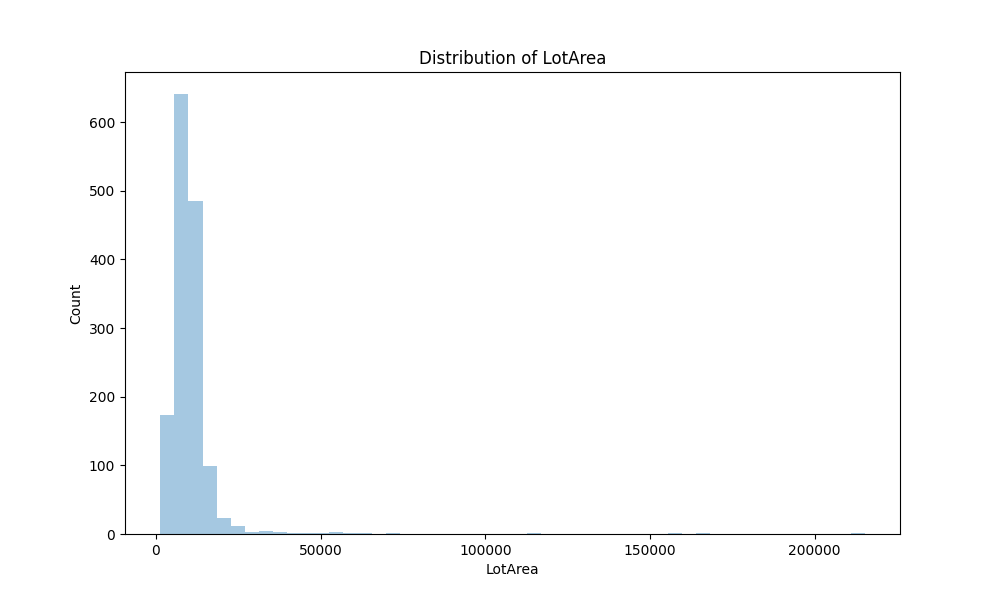
\includegraphics[width=\textwidth]{../hw1/img/Part_I/LotArea.png}
        \caption{Distribution of \texttt{LotArea}}
    \end{subfigure}
    \hfill
    \begin{subfigure}[b]{0.9\textwidth}
        \centering
        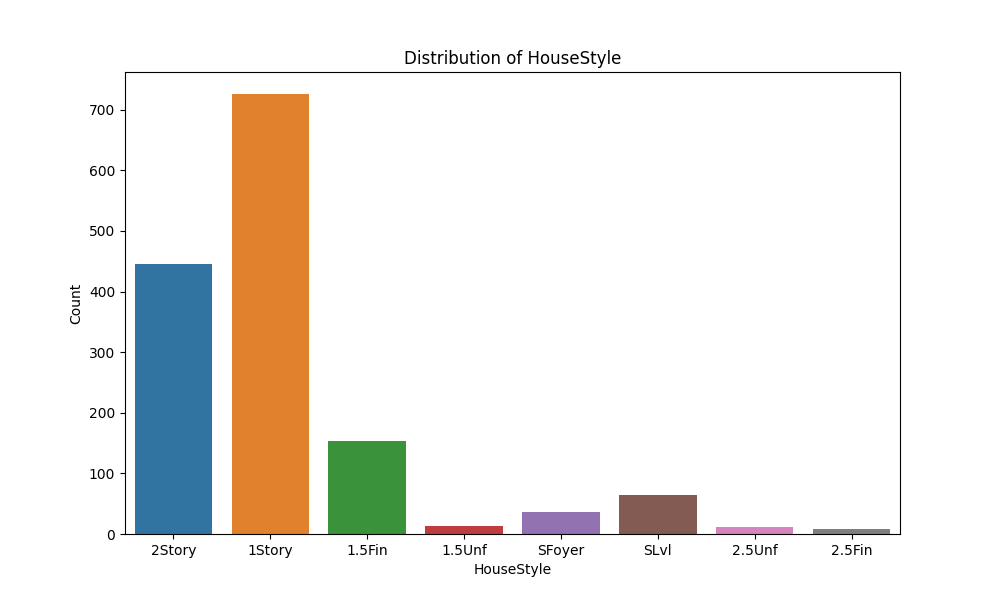
\includegraphics[width=\textwidth]{../hw1/img/Part_I/HouseStyle.png}
        \caption{Distribution of \texttt{HouseStyle}}
    \end{subfigure}
    \caption{Distribution of \texttt{LotArea} and \texttt{HouseStyle} features}
    \label{fig:feature_distribution}
\end{figure}

\subsubsection{Data preprocessing steps}

\textbf{Feature selection}: 

(This step has been conducted by discussion with Tian Jin from the same class.) Based on the data description, we can identify the features that best represent the relationship. By doing so, we can filter out the features that do not make big impact on people's decision on house purchase. For example, the \texttt{Street} feature is removed as it has only two values to represent the type of road access to the property, which is not likely to influence the decision. The selected features are shown in Listing \ref{lst:feature_selection}.

\begin{lstlisting}[language=Python, label={lst:feature_selection}, caption={Features selected with human knowledge}]
    num_features_to_keep = [
        "LotFrontage", "LotArea", "OverallQual",
        "OverallCond", "YearBuilt", "YearRemodAdd",
        "MasVnrArea", "TotalBsmtSF", "GrLivArea",
        "BsmtFullBath", "BsmtHalfBath", "FullBath",
        "HalfBath", "BedroomAbvGr", "KitchenAbvGr",
        "TotRmsAbvGrd", "Fireplaces", "GarageArea",
        "PoolArea", "YrSold",
    ]

    cat_features_to_keep = [
        "MSZoning", "Utilities", "LandSlope",
        "BldgType", "HouseStyle", "ExterQual",
        "ExterCond", "BsmtQual", "BsmtCond",
        "HeatingQC", "CentralAir", "KitchenQual",
        "FireplaceQu", "GarageQual", "GarageCond",
        "PoolQC", "SaleType",
    ]
\end{lstlisting}

\textbf{Handling missing values}: 

Handling missing values is a critical step in the data preprocessing, ensuring data completeness and accuracy; my approach involves dropping features with over 50\% missing values, and for categorical attributes, I will impute missing values using the mode, while for numerical features, I will employ the mean as the imputation strategy.

The code in Listing \ref{lst:detecting_fea_high_na} is drop features with high amount of missing values. The features with over 50\% missing values are dropped since they are not likely to provide useful information. Those features include \texttt{FireplaceQu}, \texttt{PoolQC}.

\begin{lstlisting}[language=Python, label={lst:detecting_fea_high_na}, caption={Drop the features with high amount of missing values}]
def get_feature_to_drop_by_hight_na(df_train, feature_list, threshold):
    null_counts = df_train.loc[:, feature_list].isna().sum() / len(df_train)
    return list(null_counts[null_counts > threshold].index)

features_to_drop_by_hight_na = get_feature_to_drop_by_hight_na(
    df, df.columns, threshold=0.5)
print(f"Features to drop: {features_to_drop_by_hight_na}")
df = df.drop(features_to_drop_by_hight_na, axis=1)
\end{lstlisting}

One thing to be noted is that the missing value should be filled with the mode/mean of that feature in the training data, instead of the whole dataset. This is because the test data should not be used to influence the training process. The code in Listing \ref{lst:impute_missing_values} is used to impute the missing values in the dataset.

\begin{lstlisting}[language=Python, label={lst:impute_missing_values}, caption={Fill the missing values with the measures of the feature in the training data}]
# Get the mathematical measures of each feature
def get_fea_measures_dict(df_train, feature_list, measure="mode"):
    measure_dict = dict()
    for col in feature_list:
        if measure == "mode":
            measure_dict[col] = df_train[col].mode()[0]
        elif measure == "mean":
            measure_dict[col] = df_train[col].mean()
        elif measure == "median":
            measure_dict[col] = df_train[col].median()
        else:
            raise ValueError("measure should be mode/mean/median")
    return measure_dict

cat_mode_dict = get_fea_measures_dict(df, cat_features, "mode")
num_mean_dict = get_fea_measures_dict(df, num_features, "mean")

# Fill the NA values in categorical/numerical features with the mode/mean of the features in the training dataset
def fill_na_with_measures(df, measure_dict):
    """
    Fill the NA values in features with the measures of the features in the training dataset

    Args:
        df: a Pandas dataframe containing the data to be transformed
        measure_dict: a dict containing the measure of each feature

    Return:
        A Pandas dataframe after NA values being filled
    """
    for col in measure_dict.keys():
        df[col].fillna(measure_dict[col], inplace=True)
    return df

df = fill_na_with_measures(df, cat_mode_dict)
df = fill_na_with_measures(df, num_mean_dict)
\end{lstlisting}

\textbf{Transforming ordinal features}:

Transforming ordinal features, originally categorical, into numerical representations allows us to capture and utilize the inherent order and hierarchy within these features for more meaningful analysis and modeling, enhancing our understanding of the data's relationships. Consequently, there are several ordinal features within the categorical variables, and our next step involves converting them into numerical representations. For example, all the features that contain the word "Qual" are ordinal features, as they measures the quality of certain aspects of the house. 

\begin{figure}[!htbp]
    \centering
    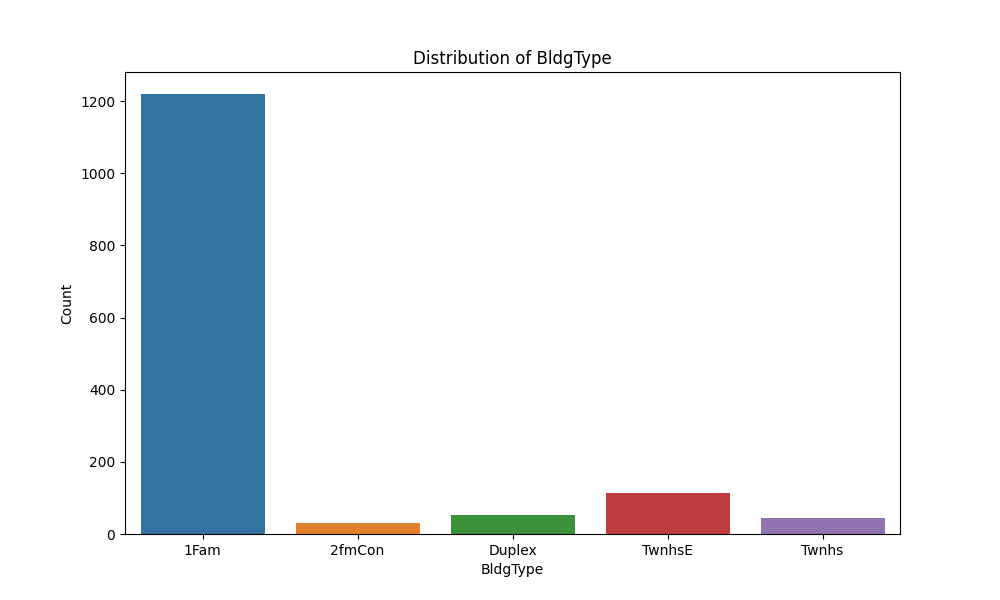
\includegraphics[width=0.9\textwidth]{../hw1/img/Part_I/BldgType.png}
    \caption{Distribution of \texttt{BldgType}}
    \label{fig:bldgtype}
\end{figure}

\textbf{Dropping highly-skewed features}:

Dropping highly-skewed features is essential because they do not provide valuable information and can potentially introduce noise into our analysis; as a result, we will remove these skewed features in the following steps. The code in Listing \ref{lst:drop_skewed_features} is used to drop the features with high skewness. It turned out that most of the categorical features remaining in the dataset are highly skewed, so I decided to drop all of them except for \texttt{HouseStyle}. For example, Figure \ref{fig:bldgtype} shows the skewness of the \texttt{BldgType} feature.

\begin{lstlisting}[language=Python, label={lst:drop_skewed_features}, caption={Drop the features with high skewness}]
def get_skewed_features(df, feature_list, threshold=0.7):
    skewed_features = list()
    for col in feature_list:
        if df[col].value_counts(normalize=True).values[0] > threshold:
            skewed_features.append(col)
    return skewed_features

feature_to_drop_skewed = get_skewed_features(df, cat_features)
print(f"Features to drop: {feature_to_drop_skewed}")
df = df.drop(feature_to_drop_skewed, axis=1)
\end{lstlisting}

\textbf{One-hot encoding}:

One-hot encoding is a common technique used to transform categorical features into numerical representations. It is a process of converting categorical features into a vector representation that can be easily used by machine learning algorithms. The code in Listing \ref{lst:one_hot_encoding} is used to one-hot encode the categorical features.

\begin{lstlisting}[language=Python, label={lst:one_hot_encoding}, caption={One-hot encode the categorical features}]
# Create a dict containing all the feature names of each categorical feature
def get_categories_list(df_train, categorical_features):
    categories = dict()
    for col in categorical_features:
        categories[col] = df_train[col].unique().tolist()
    return categories

# Perform one-hot encoding to the training dataset
def apply_one_hot_encode(df, categories_dict):
    for col, categories in categories_dict.items():
        for category in categories:
            df[f"{col}_{category}"] = (df[col] == category).astype(int)
        df.drop(col, axis=1, inplace=True)
    return df

categories_dict = get_categories_list(df, cat_features)
df = apply_one_hot_encode(df, categories_dict)
\end{lstlisting}

\begin{figure}[!htbp]
    \centering
    \begin{subfigure}[b]{0.49\textwidth}
        \centering
        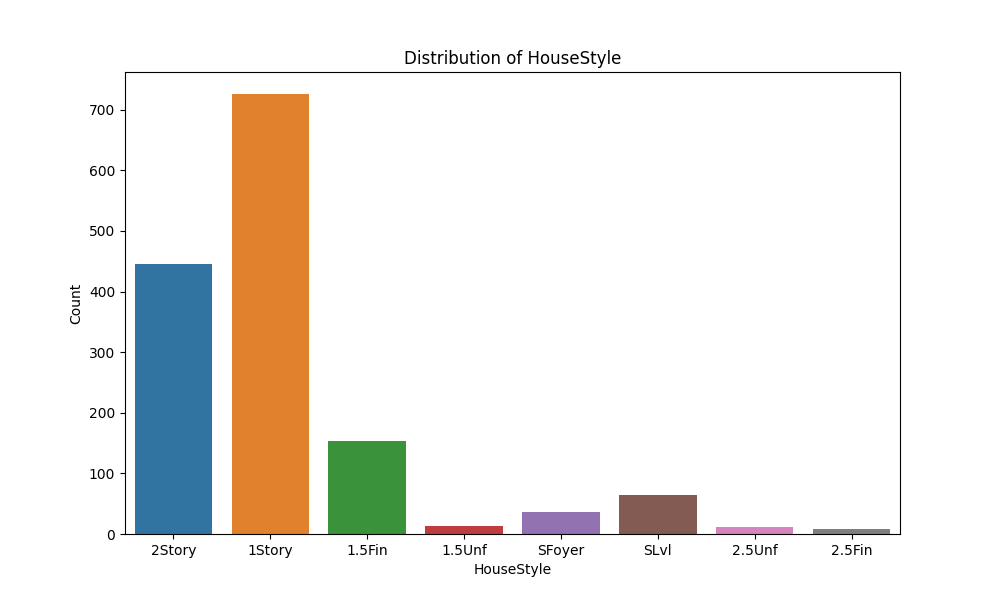
\includegraphics[width=\textwidth]{../hw1/img/Part_I/HouseStyle_before.png}
        \caption{Before one-hot encoding}
    \end{subfigure}
    \hfill
    \begin{subfigure}[b]{0.49\textwidth}
        \centering
        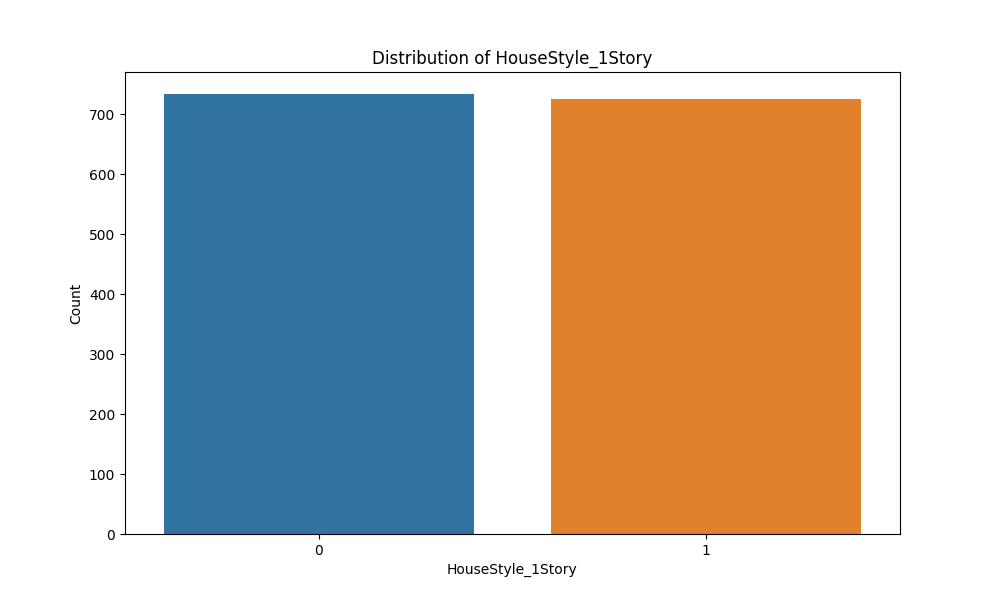
\includegraphics[width=\textwidth]{../hw1/img/Part_I/HouseStyle_after.png}
        \caption{After one-hot encoding}
    \end{subfigure}
    \caption{Distribution of \texttt{HouseStyle} before and after one-hot encoding}
    \label{fig:housestyle_before_after}
\end{figure}

In the remaining features in the dataset, \texttt{HouseStyle} is the only categorical feature that is applicable to one-hot encoding. By performing one-hot encoding, we can not only transform the categorical feature into numerical representations, but also avoid introducing the order of the categories of \texttt{HouseStyle} into the model. Figure \ref{fig:housestyle_before_after} shows the distribution of the \texttt{HouseStyle} feature before and after one-hot encoding. It can be seen that the distribution of the feature is not skewed after one-hot encoding.

\textbf{Feature scaling}:

Feature scaling is necessary to ensure that all the features in a dataset have similar scales or ranges, as many machine learning algorithms are sensitive to the magnitude of feature values. The code in Listing \ref{lst:feature_scaling} is used to scale the numerical features in the dataset.

\begin{lstlisting}[language=Python, label={lst:feature_scaling}, caption={Scale the numerical features in the dataset}]
from sklearn.preprocessing import Normalizer
X_normalized = Normalizer().fit_transform(df)
\end{lstlisting}

\subsubsection{Ordinary least squares (OLS): training and testing}

The code in Listing \ref{lst:ols} is used to implement the OLS model without Scikit-learn:

\begin{lstlisting}[language=Python, label={lst:ols}, caption={OLS implementation}]
# Compute OLS from scratch
def OLS(X, Y):
    theta = np.linalg.inv(X.T.dot(X)).dot(X.T).dot(Y)
    return theta

# Fit the model
theta = OLS(X_normalized, target)

# Inference
pred = X_normalized.dot(theta)
\end{lstlisting}

The mean squared error (MSE) of the OLS model is 974304111.65, and the \(R^2\) score is 0.69103. After training the model, the test set is loaded and preprocessed in the same way as the training set. Then, the model is used to predict the survival of passengers in the test set. The predictions are saved in a CSV file and submitted to Kaggle. The public score on the test set is 1.24275, which is ranked 3,890 out of 3.985 teams on the leaderboard as in Figure \ref{fig:kaggle_leaderboard_1}.

% Kaggle leaderboard
\begin{figure}[!htbp]
    \centering
    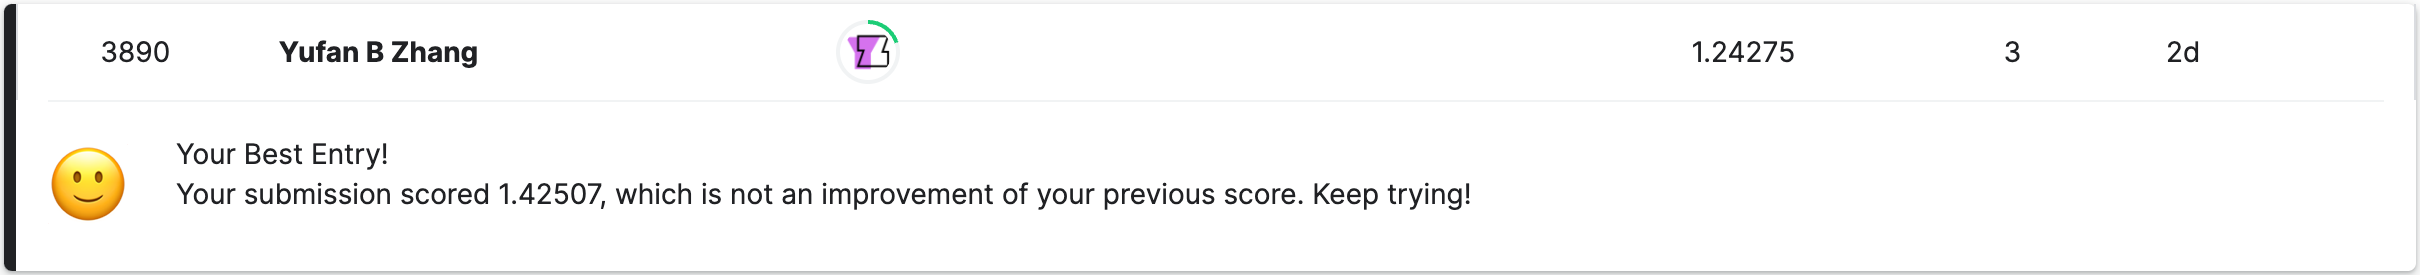
\includegraphics[width=\textwidth]{../hw1/result/Part_I/leaderboard.png}
    \caption{My Submission on Kaggle leaderboard}
    \label{fig:kaggle_leaderboard_1}
\end{figure}

\subsection{The Titanic Disaster}

\subsubsection{Data preprocessing steps}

First, two features that do not provide any useful information are removed from the dataset: \texttt{Ticket} and \texttt{Name}. Then, the feature with more than 50\% missing values, \texttt{Cabin}, is also removed. By doing so, I can reduce the feature space to 9 features:

\begin{lstlisting}[language=Python]
['Pclass', 'Age', 'SibSp', 'Parch', 'Fare', 'Sex', 'Embarked']
\end{lstlisting}

Next, each remaining feature is examined to see if its own distribution, its correlation with the target variable, or its correlation with other features can provide any useful information. This step is highly motivated by Titanic Data Science Solutions on Kaggle.

\begin{figure}[!htbp]
    \centering
    \begin{subfigure}[b]{0.49\textwidth}
        \centering
        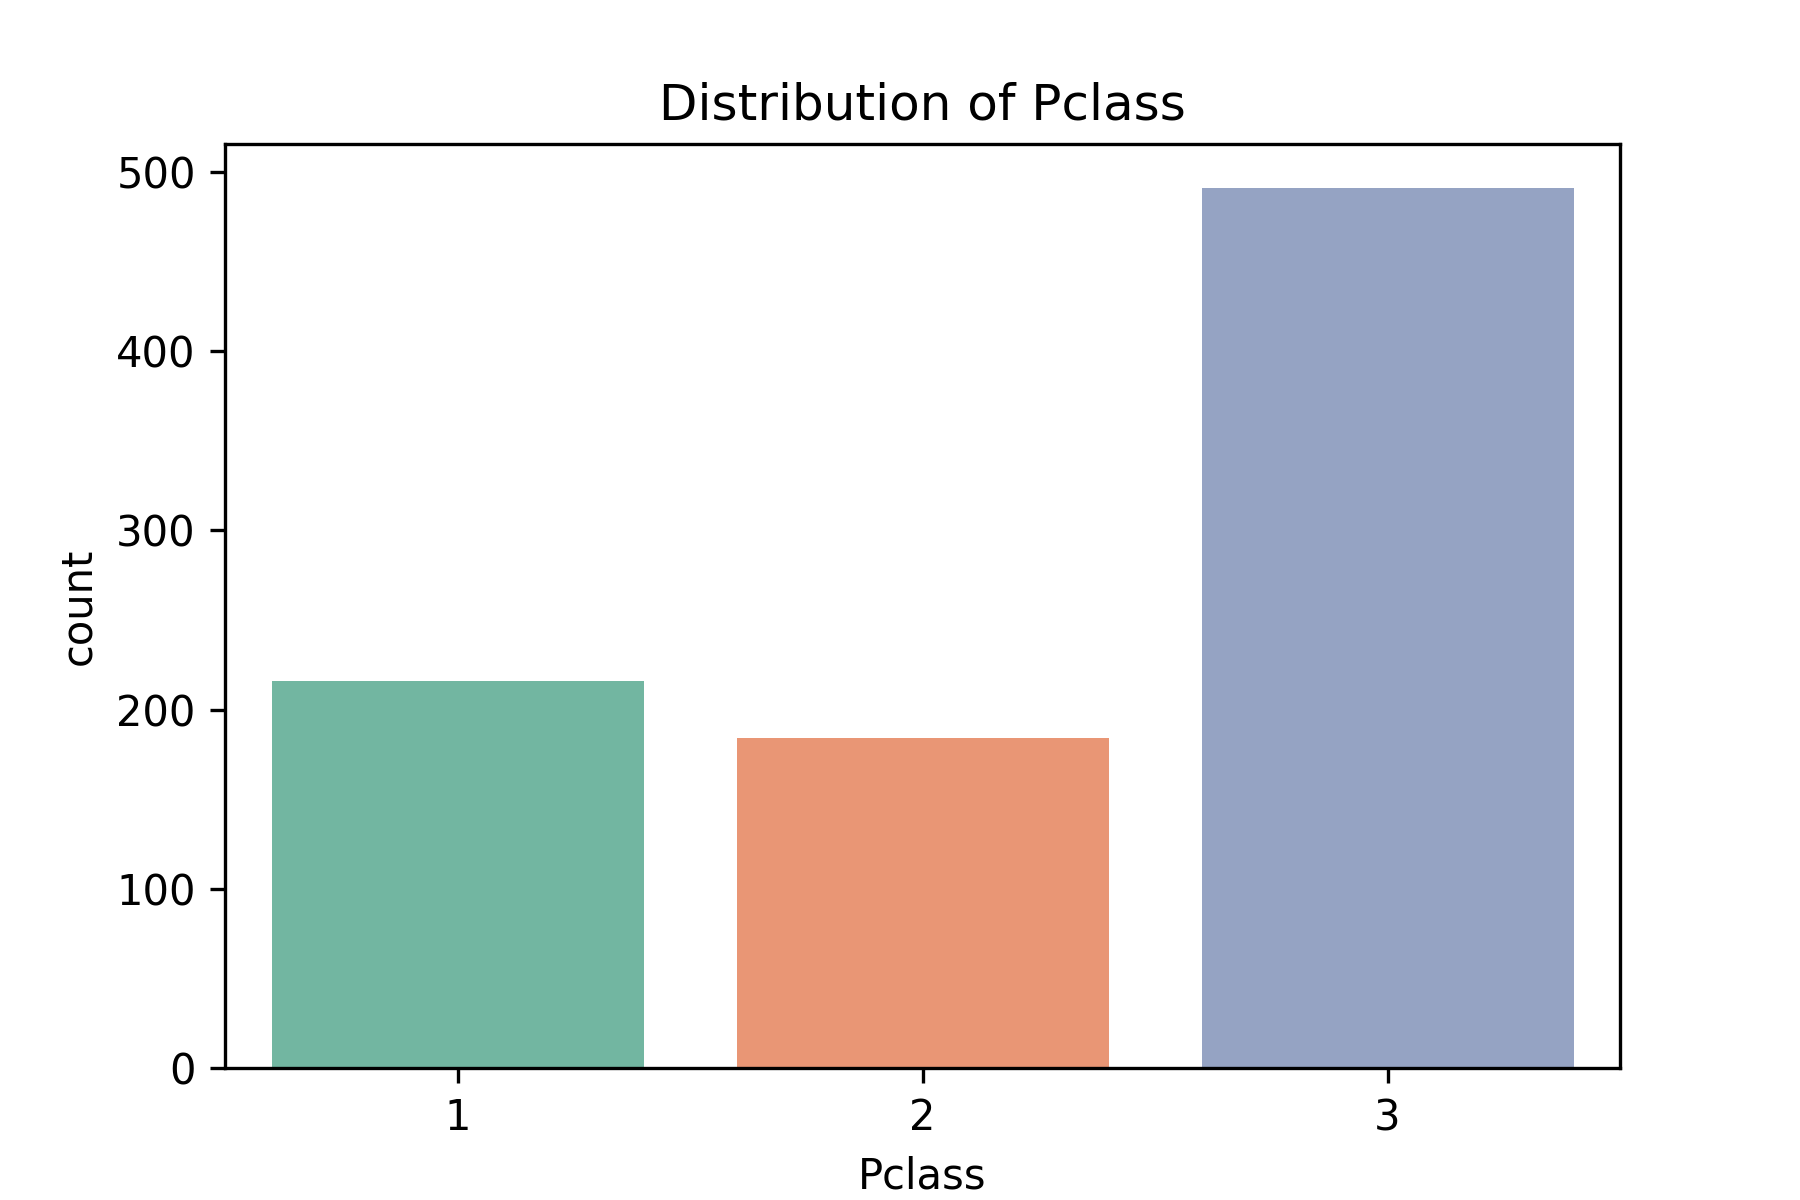
\includegraphics[width=\textwidth]{../hw1/img/Part_II/distribution_of_pclass.png}
        \caption{Distribution of \texttt{Pclass}}
        \label{fig:pclass_distribution}
    \end{subfigure}
    \hfill
    \begin{subfigure}[b]{0.49\textwidth}
        \centering
        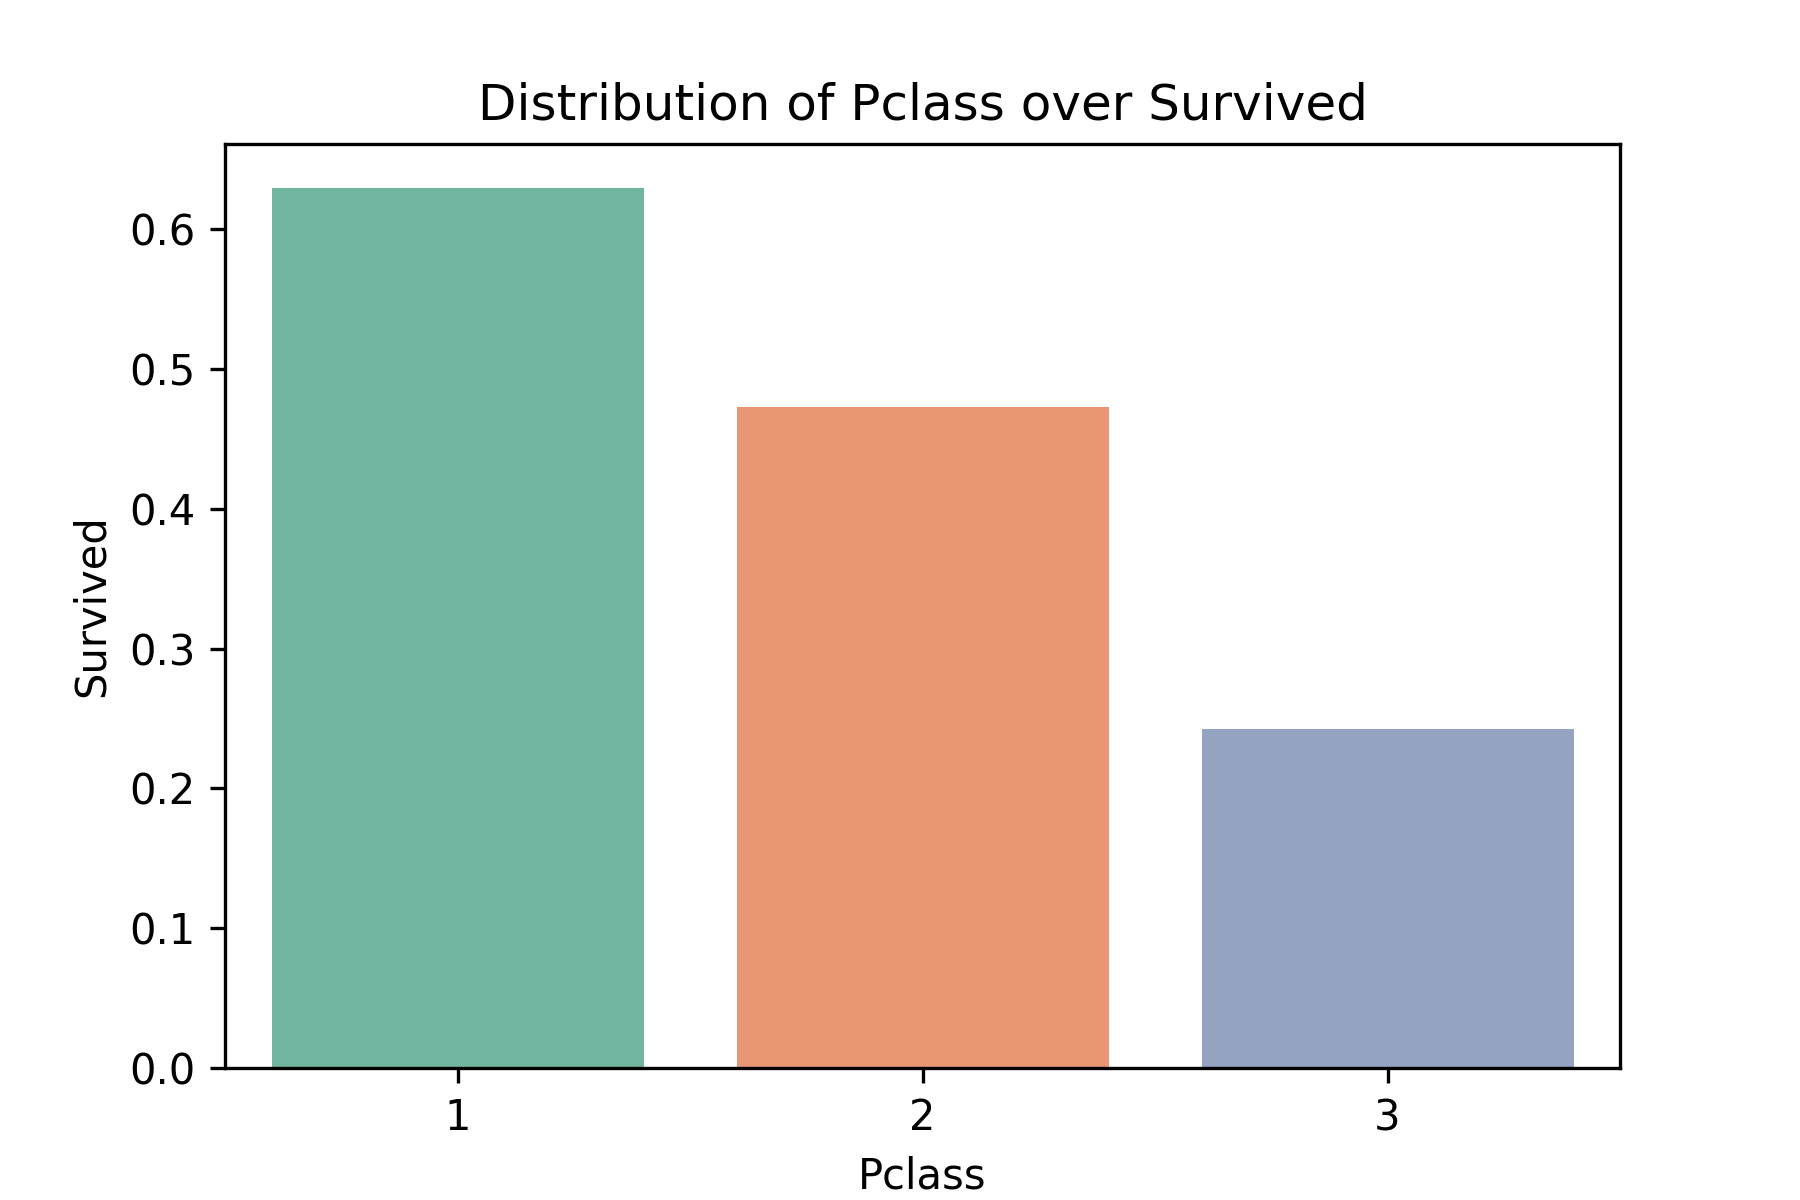
\includegraphics[width=\textwidth]{../hw1/img/Part_II/distribution_of_pclass_over_survived.png}
        \caption{Distribution of \texttt{Survived} over \texttt{Pclass}}
        \label{fig:pclass_vs_survived}
    \end{subfigure}
    \caption{Distribution of \texttt{Pclass} and its correlation with \texttt{Survived}}
    \label{fig:pclass}
\end{figure}

\textbf{Pclass:} The distribution of \texttt{Pclass} is shown in Figure \ref{fig:pclass}. It can be seen that the majority of the passengers are in class 3, followed by class 1 and class 2. Also, the survival rate of passengers in class 1 is higher than that of passengers in class 2, which is higher than that of passengers in class 3. Therefore, this feature is kept and does not need to be one-hot encoded as the numerical values already represent the order of the classes.

\begin{figure}[!htbp]
    \centering
    \begin{subfigure}[b]{0.49\textwidth}
        \centering
        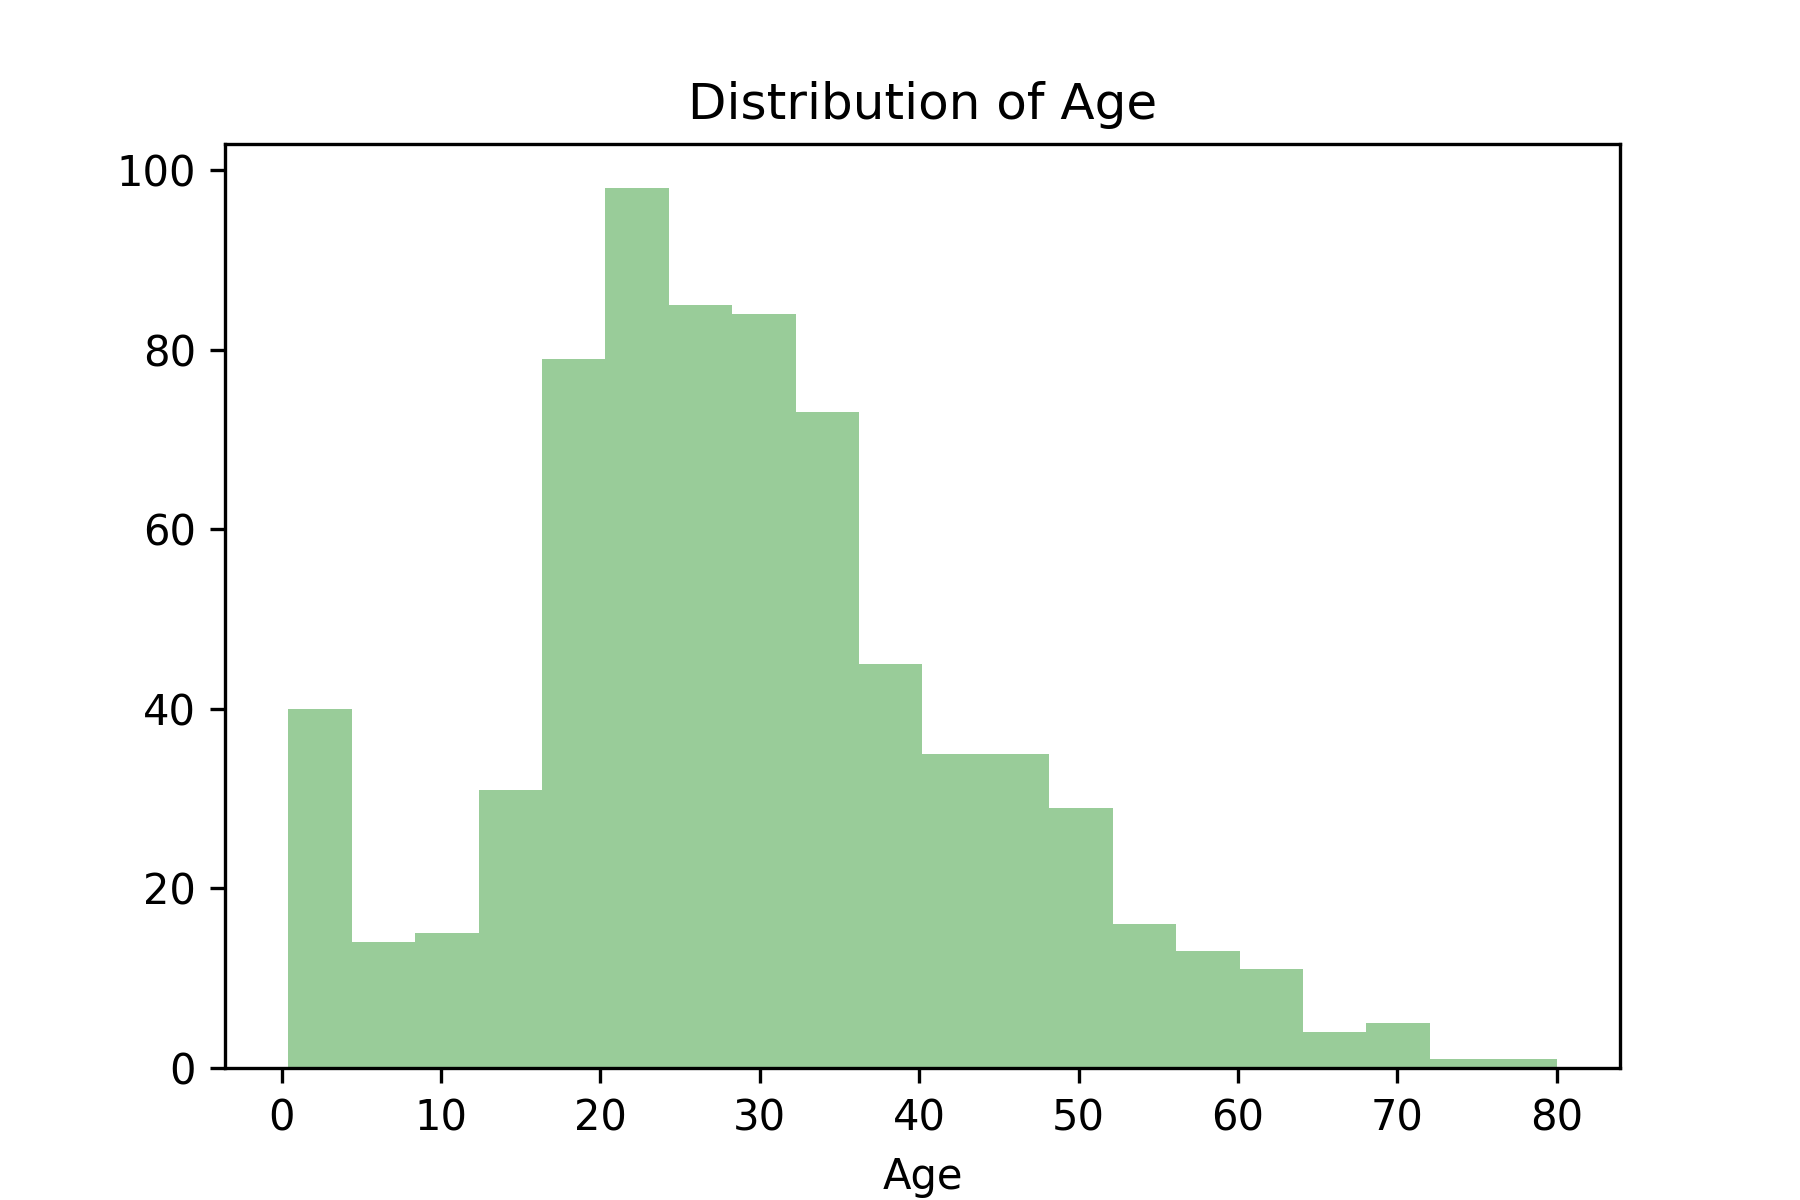
\includegraphics[width=\textwidth]{../hw1/img/Part_II/distribution_of_age.png}
        \caption{Distribution of \texttt{Age}}
        \label{fig:age_distribution}
    \end{subfigure}
    \hfill
    \begin{subfigure}[b]{0.49\textwidth}
        \centering
        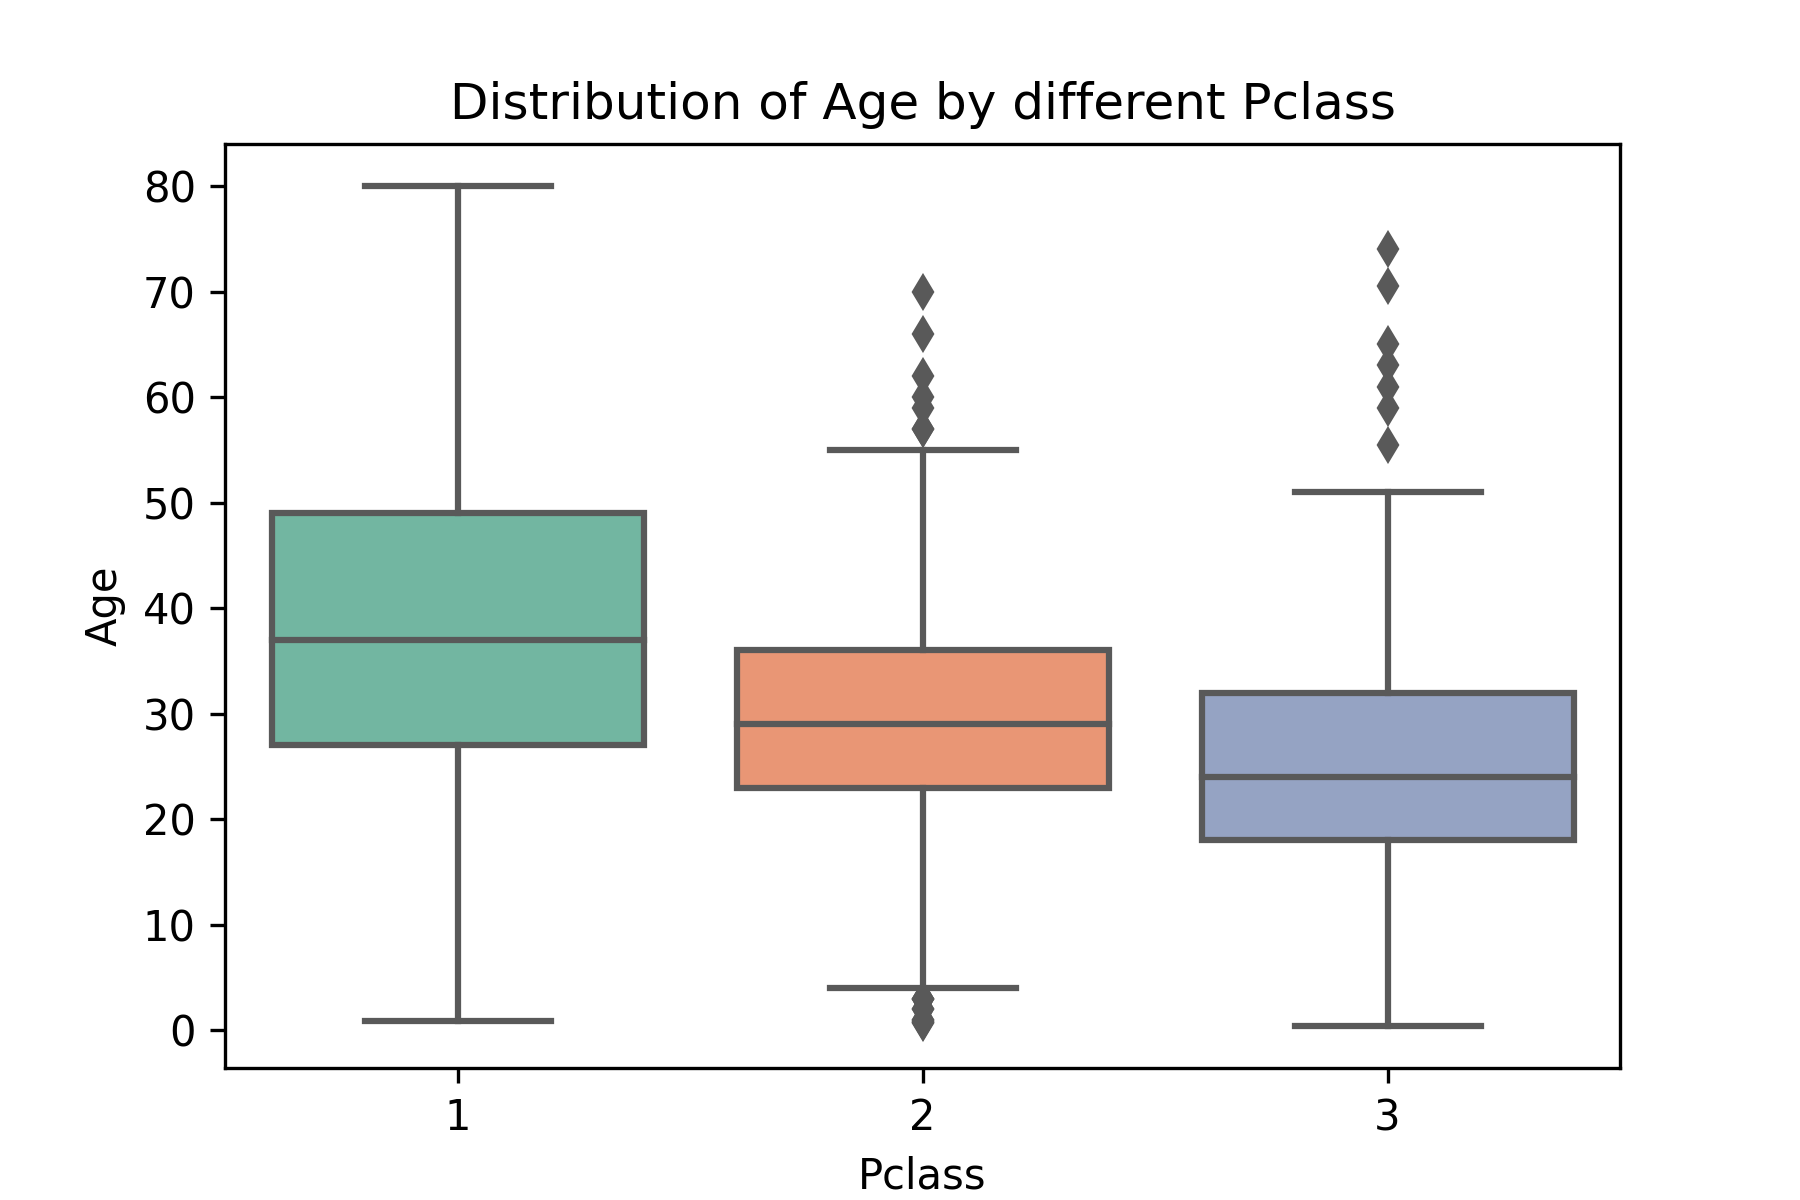
\includegraphics[width=\textwidth]{../hw1/img/Part_II/distribution_of_age_by_pclass.png}
        \caption{Distribution of \texttt{Age} over \texttt{Pclass}}
        \label{fig:age_vs_pclass}
    \end{subfigure}
    \begin{subfigure}[b]{0.49\textwidth}
        \centering
        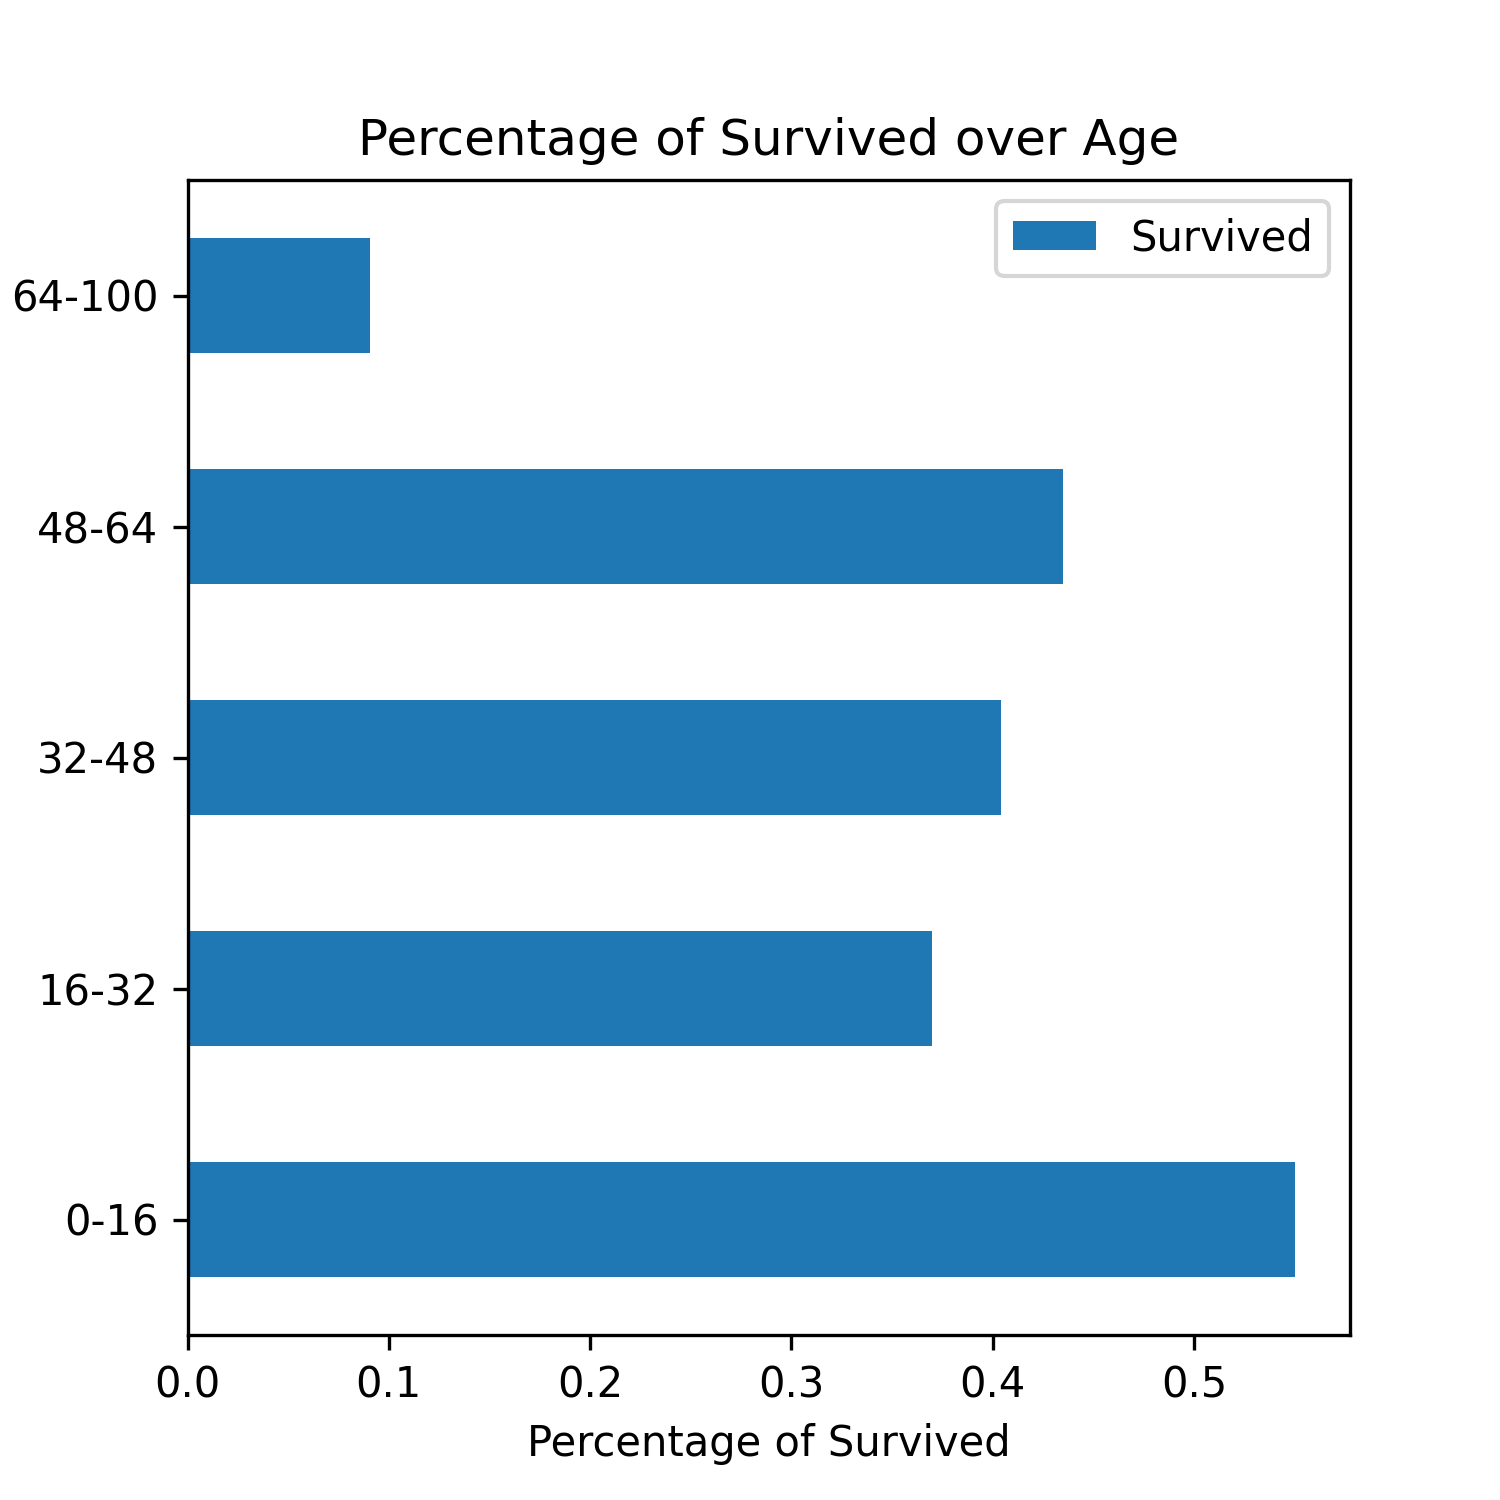
\includegraphics[width=\textwidth]{../hw1/img/Part_II/percentage_of_survived_over_age_group.png}
        \caption{Distribution of \texttt{Age} over \texttt{Pclass}}
        \label{fig:age_groups_vs_survived}
    \end{subfigure}
    \begin{subfigure}[b]{0.49\textwidth}
        \centering
        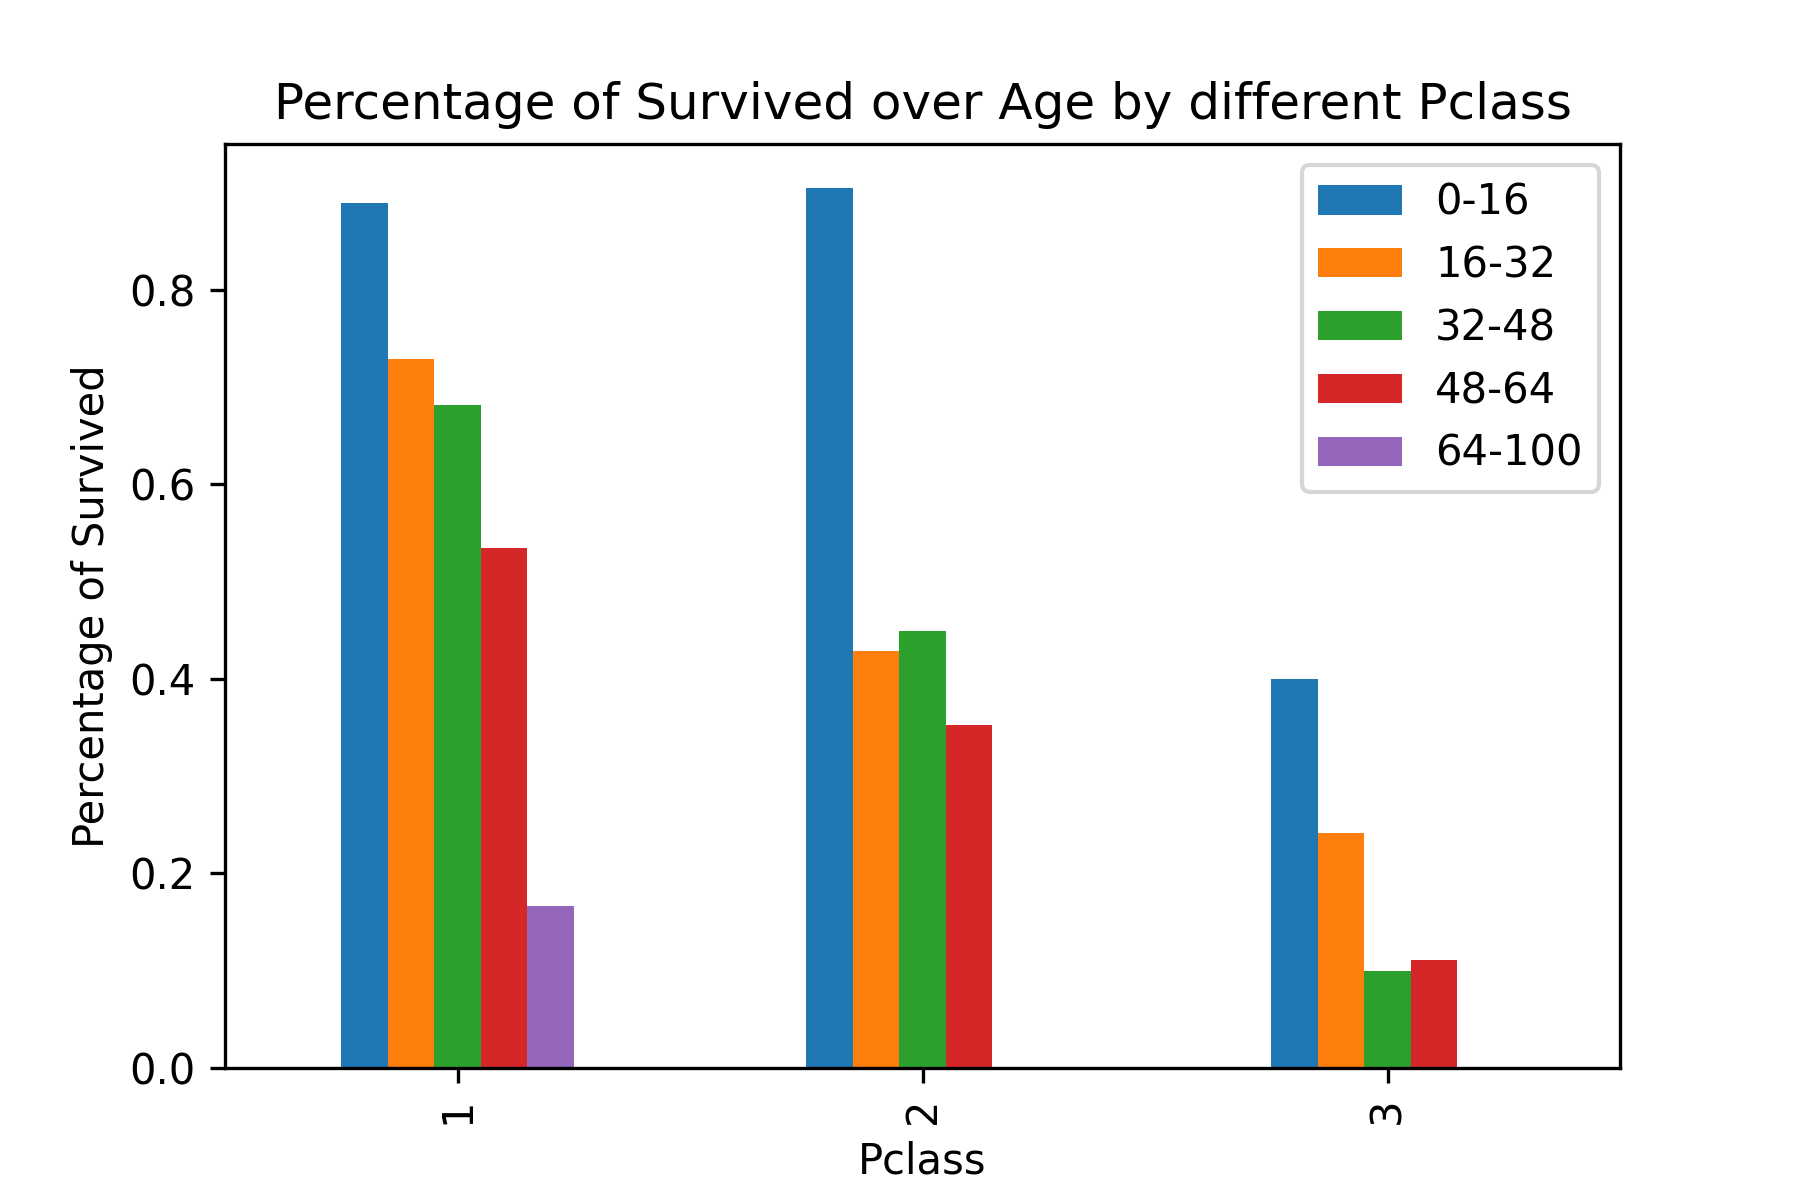
\includegraphics[width=\textwidth]{../hw1/img/Part_II/percentage_of_survived_over_age_by_pclass.png}
        \caption{Distribution of \texttt{Survived} of each age group over \texttt{Pclass}}
        \label{fig:age_groups_vs_survived_by_pclass}
    \end{subfigure}
    \caption{Distribution of \texttt{Age} and its correlation with \texttt{Survived} and \texttt{Pclass}}
    \label{fig:age}
\end{figure}

\textbf{Age:} As illustrated in Figure \ref{fig:age}, it was noted that there are 177 (19.865\%) missing values within this feature, with the majority of passengers falling within the age range of 16 to 35 years. 
Furthermore, the survival rate is notably higher among passengers under 16 years old compared to those over 16 years old, and that survival rates vary across different passenger classes within distinct age groups. 
As a result of these observations, several decisions were made regarding the feature. It was determined that the feature should be retained, and the missing values should be imputed using the median age within each passenger class. 
Additionally, to enhance the feature set, new features were introduced, including \texttt{AgeGroup} 
to categorize passengers by age groups, \texttt{IsChild} to identify whether a passenger is a child (under 16 years old), and \texttt{AgeXPclass} to represent the interaction between \texttt{AgeGroup} and \texttt{Pclass}. 
Lastly, the \texttt{Age} feature was scaled to a range of [0, 1] to ensure uniformity in its values.

\textbf{SibSp \& Parch}: Both of these attributes provide information about the number of family members accompanying passengers on board the Titanic. 
The majority of passengers do not have any family members accompanying them during their voyage. 
In light of this observation, a decision has been made to introduce a new feature called \texttt{IsAlone} which will help determine whether a passenger is traveling alone or not. 
To streamline the dataset and eliminate redundancy, SibSp and Parch features has been removed, as their information can now be effectively captured by the newly created \texttt{IsAlone} feature.

\begin{figure}[!htbp]
    \centering
    \begin{subfigure}[b]{0.49\textwidth}
        \centering
        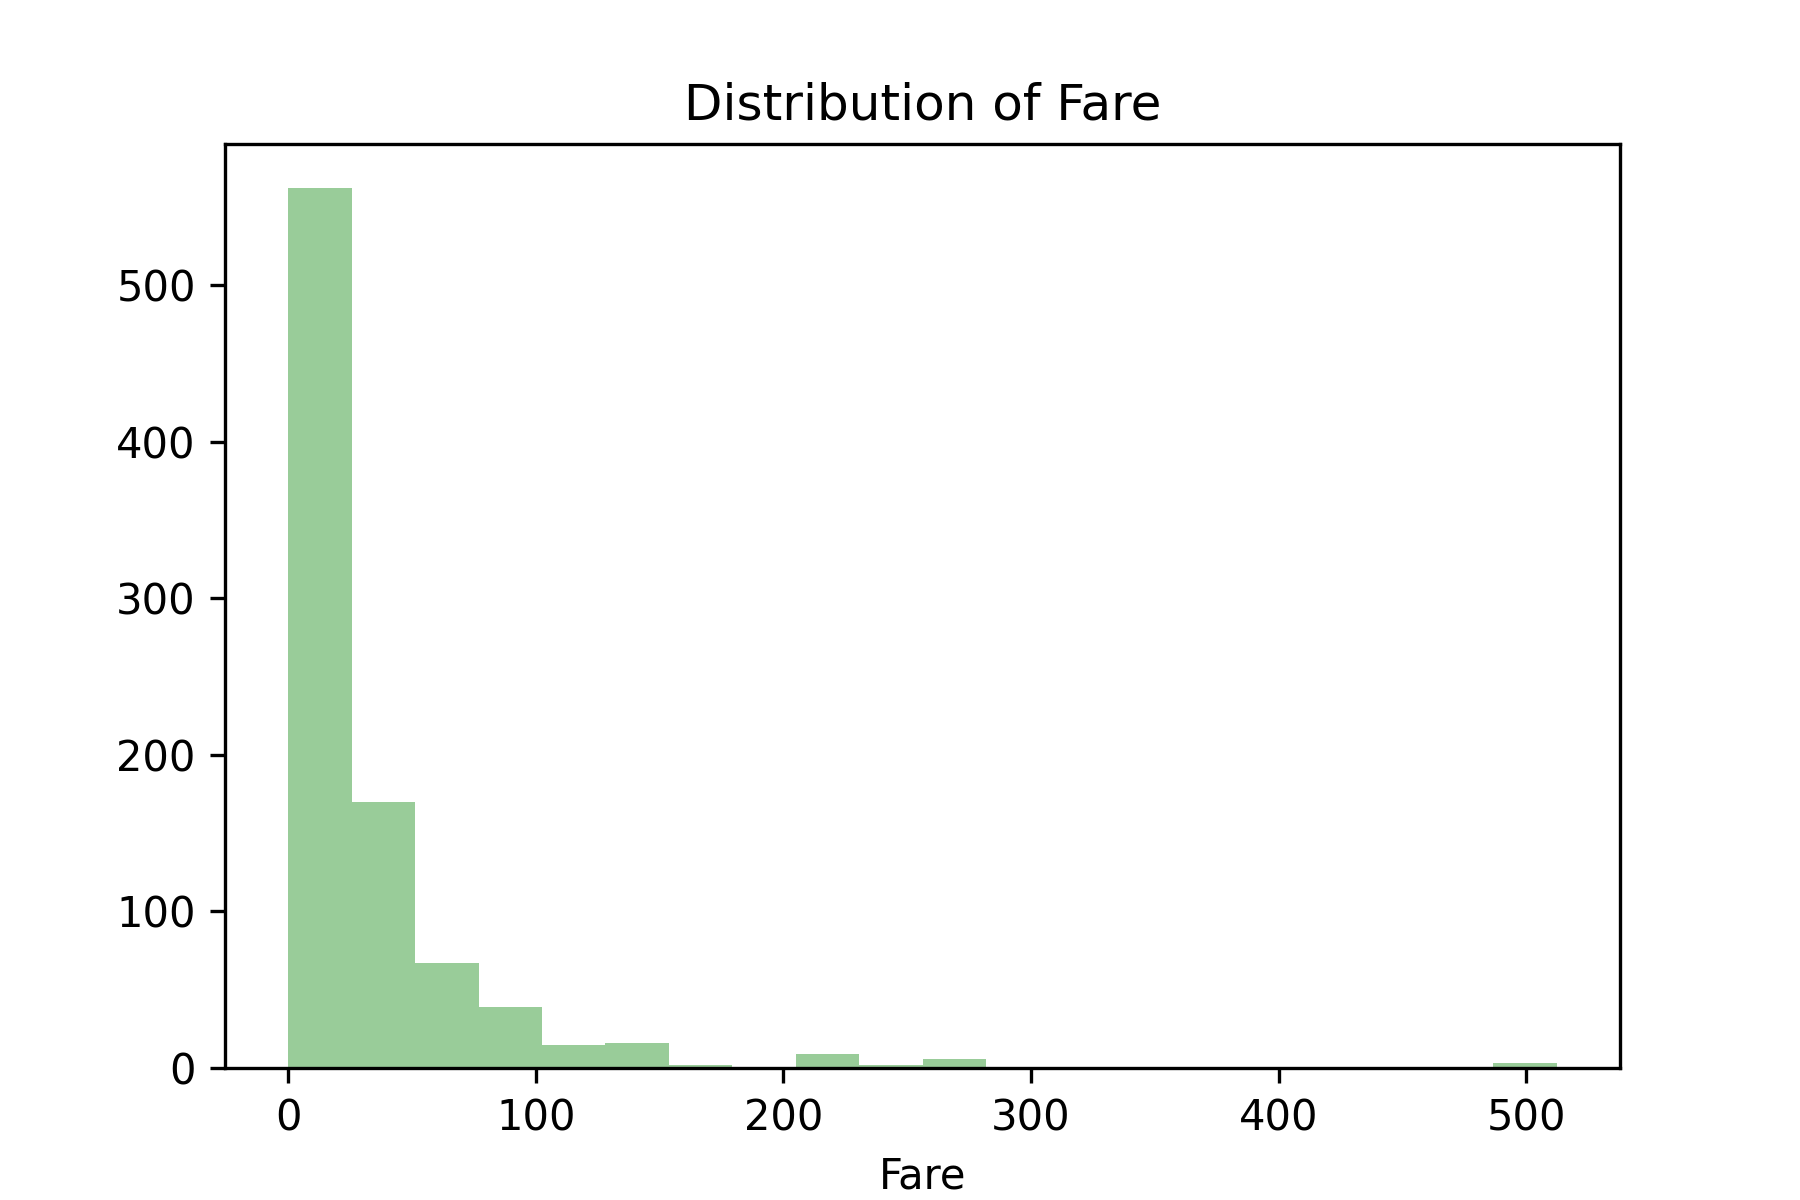
\includegraphics[width=\textwidth]{../hw1/img/Part_II/distribution_of_fare.png}
        \caption{Distribution of \texttt{Fare}}
        \label{fig:fare_distribution}
    \end{subfigure}
    \hfill
    \begin{subfigure}[b]{0.49\textwidth}
        \centering
        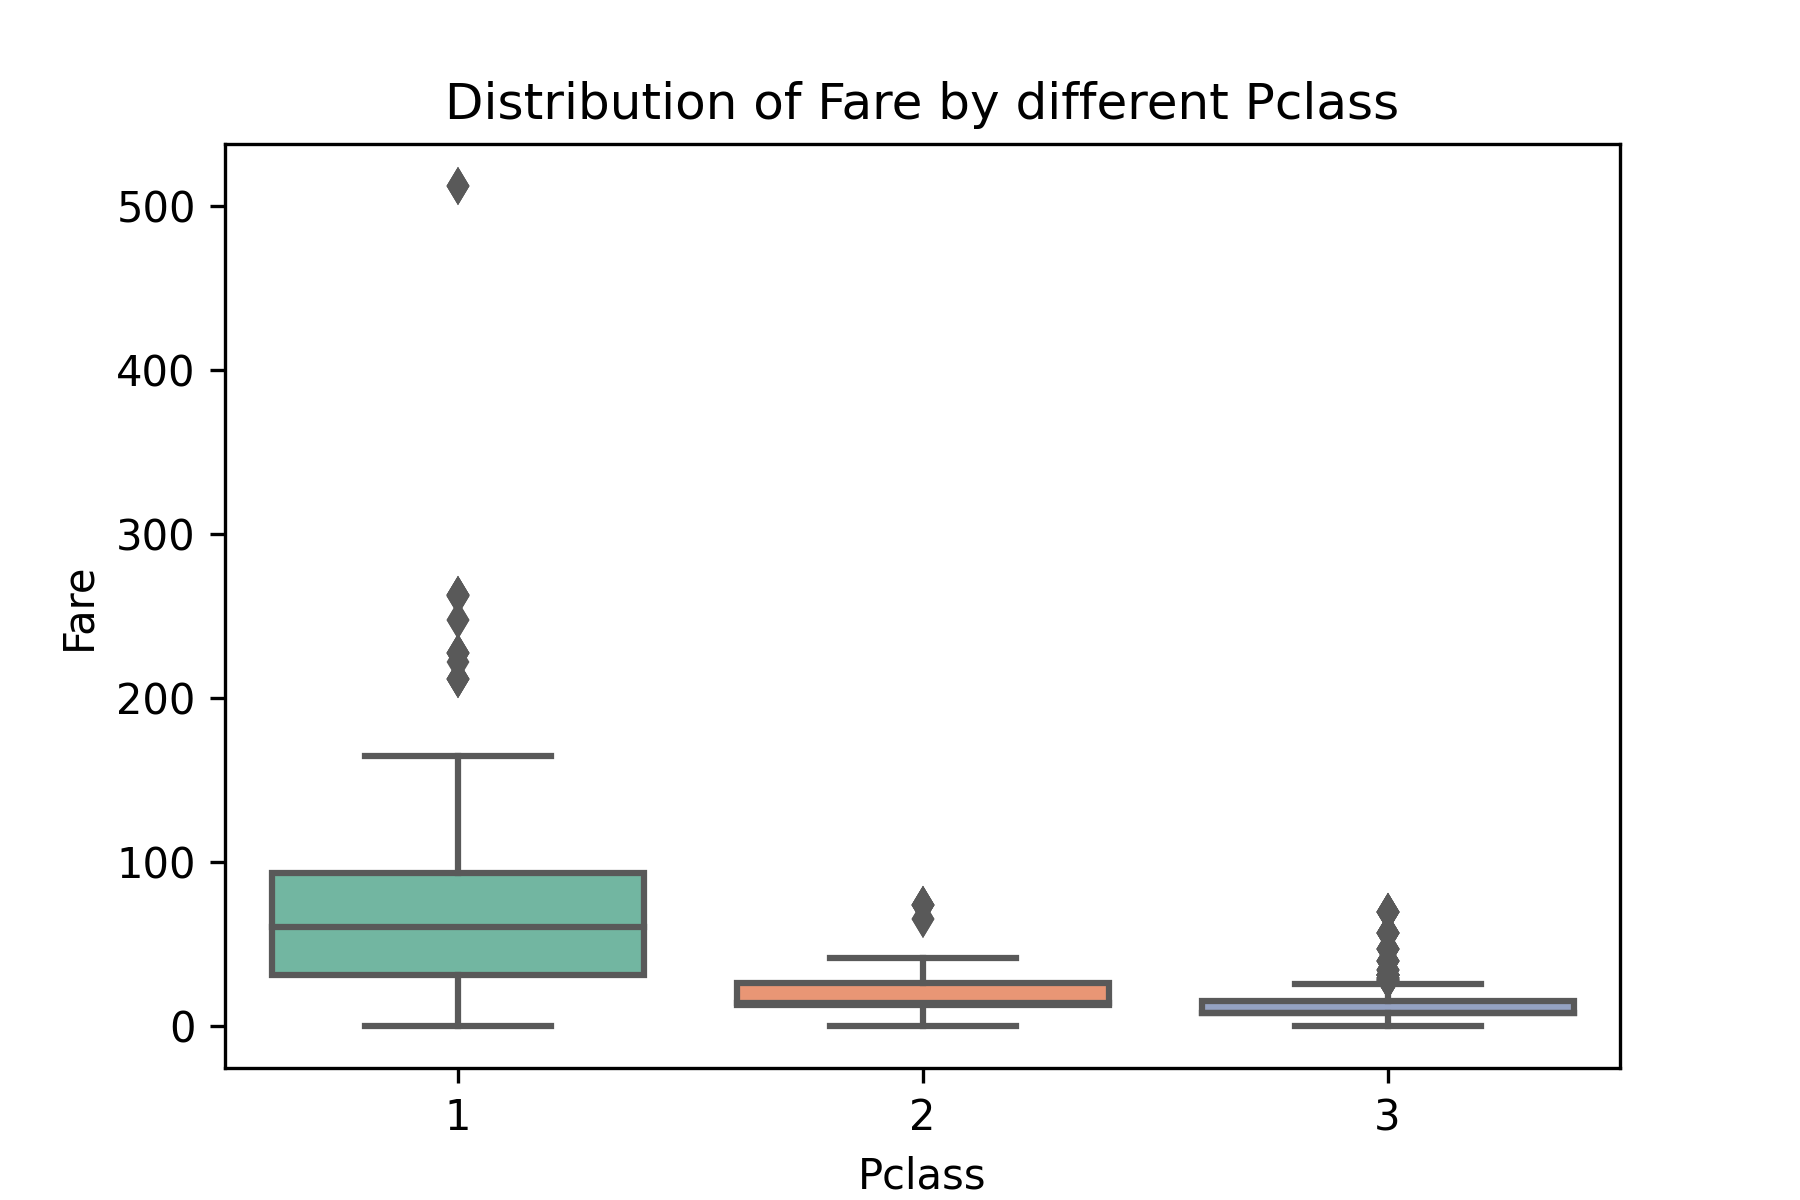
\includegraphics[width=\textwidth]{../hw1/img/Part_II/distribution_of_fare_by_pclass.png}
        \caption{Distribution of \texttt{Fare} over \texttt{Pclass}}
        \label{fig:fare_vs_pclass}
    \end{subfigure}
    \caption{Distribution of \texttt{Fare} and its correlation with \texttt{Pclass}}
    \label{fig:fare}
\end{figure}

\textbf{Fare}: There is a single missing value in this feature, which will be filled with the median fare of the corresponding Pclass, as all Pclass categories exhibit skewed distribution in terms of fare. As Figure \ref{fig:fare} shows, within the 1st class, there is an outlier with a fare value of 512.3292. To address this issue, a new feature will be introduced, \texttt{FareGroup}, to categorize passengers based on their fare. Lastly, the original \texttt{Fare} feature was dropped as part of the data preprocessing steps.

\begin{figure}[!htbp]
    \centering
    \begin{subfigure}[b]{0.49\textwidth}
        \centering
        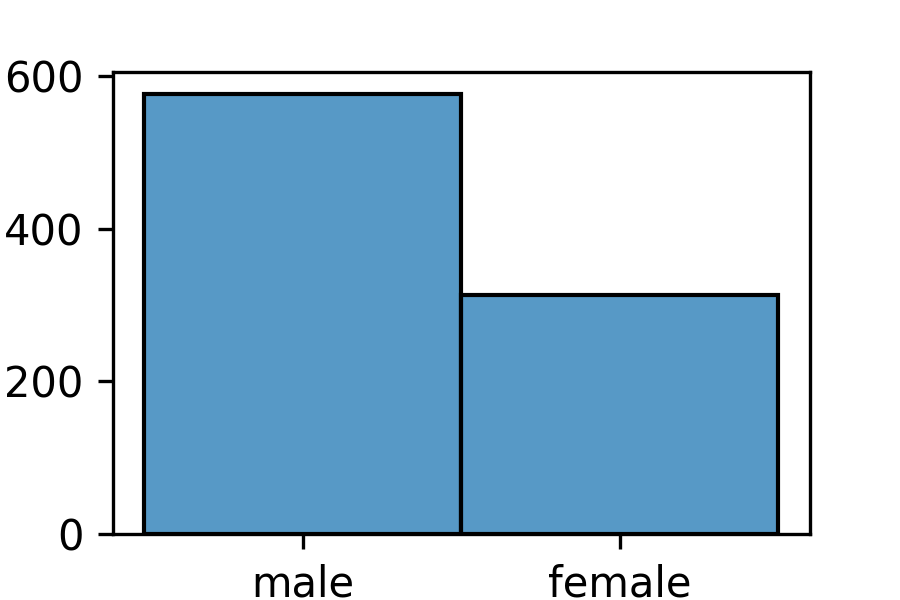
\includegraphics[width=\textwidth]{../hw1/img/Part_II/distribution_of_sex.png}
        \caption{Distribution of \texttt{Sex}}
        \label{fig:sex_distribution}
    \end{subfigure}
    \hfill
    \begin{subfigure}[b]{0.49\textwidth}
        \centering
        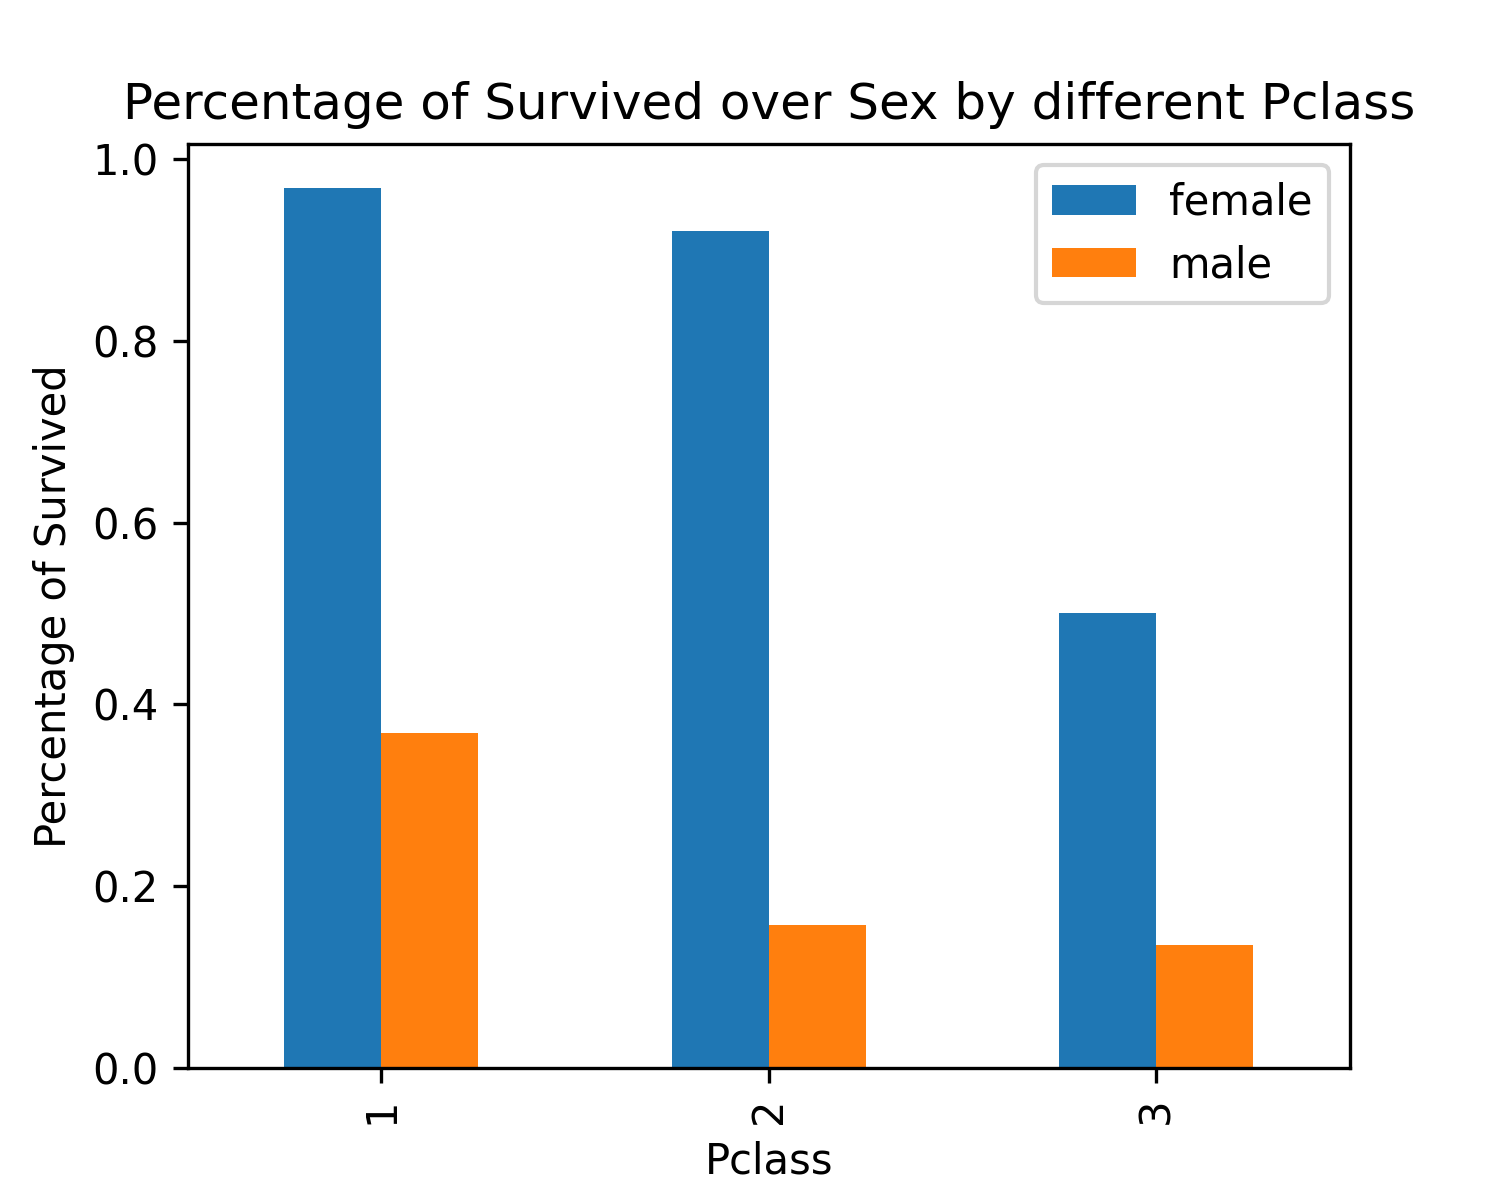
\includegraphics[width=\textwidth]{../hw1/img/Part_II/distribution_of_sex_by_pclass.png}
        \caption{Distribution of \texttt{Survived} of each Pclass group over \texttt{Sex}}
        \label{fig:sex_vs_pclass}
    \end{subfigure}
    \caption{Distribution of \texttt{Sex}}
    \label{fig:sex}
\end{figure}

\textbf{Sex}: The examination of the \texttt{Sex} feature revealed several observations, as illustrated in Figure \ref{fig:sex}. Firstly, the passenger count for males surpasses that of females aboard the ship. Secondly, the distribution of sexes among passengers in various passenger classes is relatively consistent. Additionally, it was observed that female passengers exhibit a greater likelihood of survival. Consequently, I have chosen to make the following decisions regarding this feature: convert it into a binary feature named \texttt{IsFemale}, where '1' will signify female and '0' will represent male passengers. Simultaneously, the original \texttt{Sex} feature will be dropped.

\textbf{Embarked}: Regarding the \texttt{Embarked} feature, several observations were made. Firstly, there are two missing values within this attribute. Secondly, the majority of passengers boarded from Southampton. Additionally, it was noted that the survival rate of passengers who embarked from Cherbourg is notably higher compared to those who embarked from Queenstown and Southampton. However, this discrepancy is likely influenced by the fact that a significant portion of Cherbourg's passengers belong to the 1st class. To address these observations, the missing values were filled using the most frequent value (mode) and proceed to one-hot encode this feature for further analysis.


\subsubsection{Training and testing}

For training and testing, I developed the following code to implement the logistic regression model without Scikit-learn:

\begin{lstlisting}[language=Python]
class LogisticRegression:
    def __init__(self, lr=0.01, num_iter=10000):
        self.lr = lr
        self.num_iter = num_iter
        self.theta = None

    def __sigmoid(self, z):
        return 1 / (1 + np.exp(-z))

    def __gradient(self, X, pred, y):
        return np.dot(X.T, (pred - y)) / y.size

    def fit(self, X, y):
        # Initialize the weights
        self.theta = np.zeros(X.shape[1])

        # Train the model using gradient descent
        for i in range(self.num_iter):
            z = np.dot(X, self.theta)
            pred = self.__sigmoid(z)
            gradient = np.dot(X.T, (pred - y)) / y.size
            self.theta -= self.lr * gradient

    def predict(self, X):
        z = np.dot(X, self.theta)
        pred = self.__sigmoid(z)
        return pred >= 0.5

model = LogisticRegression(lr=0.1, num_iter=150000)
model.fit(X_train, y_train)

y_pred = model.predict(X_val)
print(f"Accuracy: {accuracy_score(y_val, y_pred)}")
\end{lstlisting}

% Confusion matrix
\begin{figure}[!htbp]
    \centering
    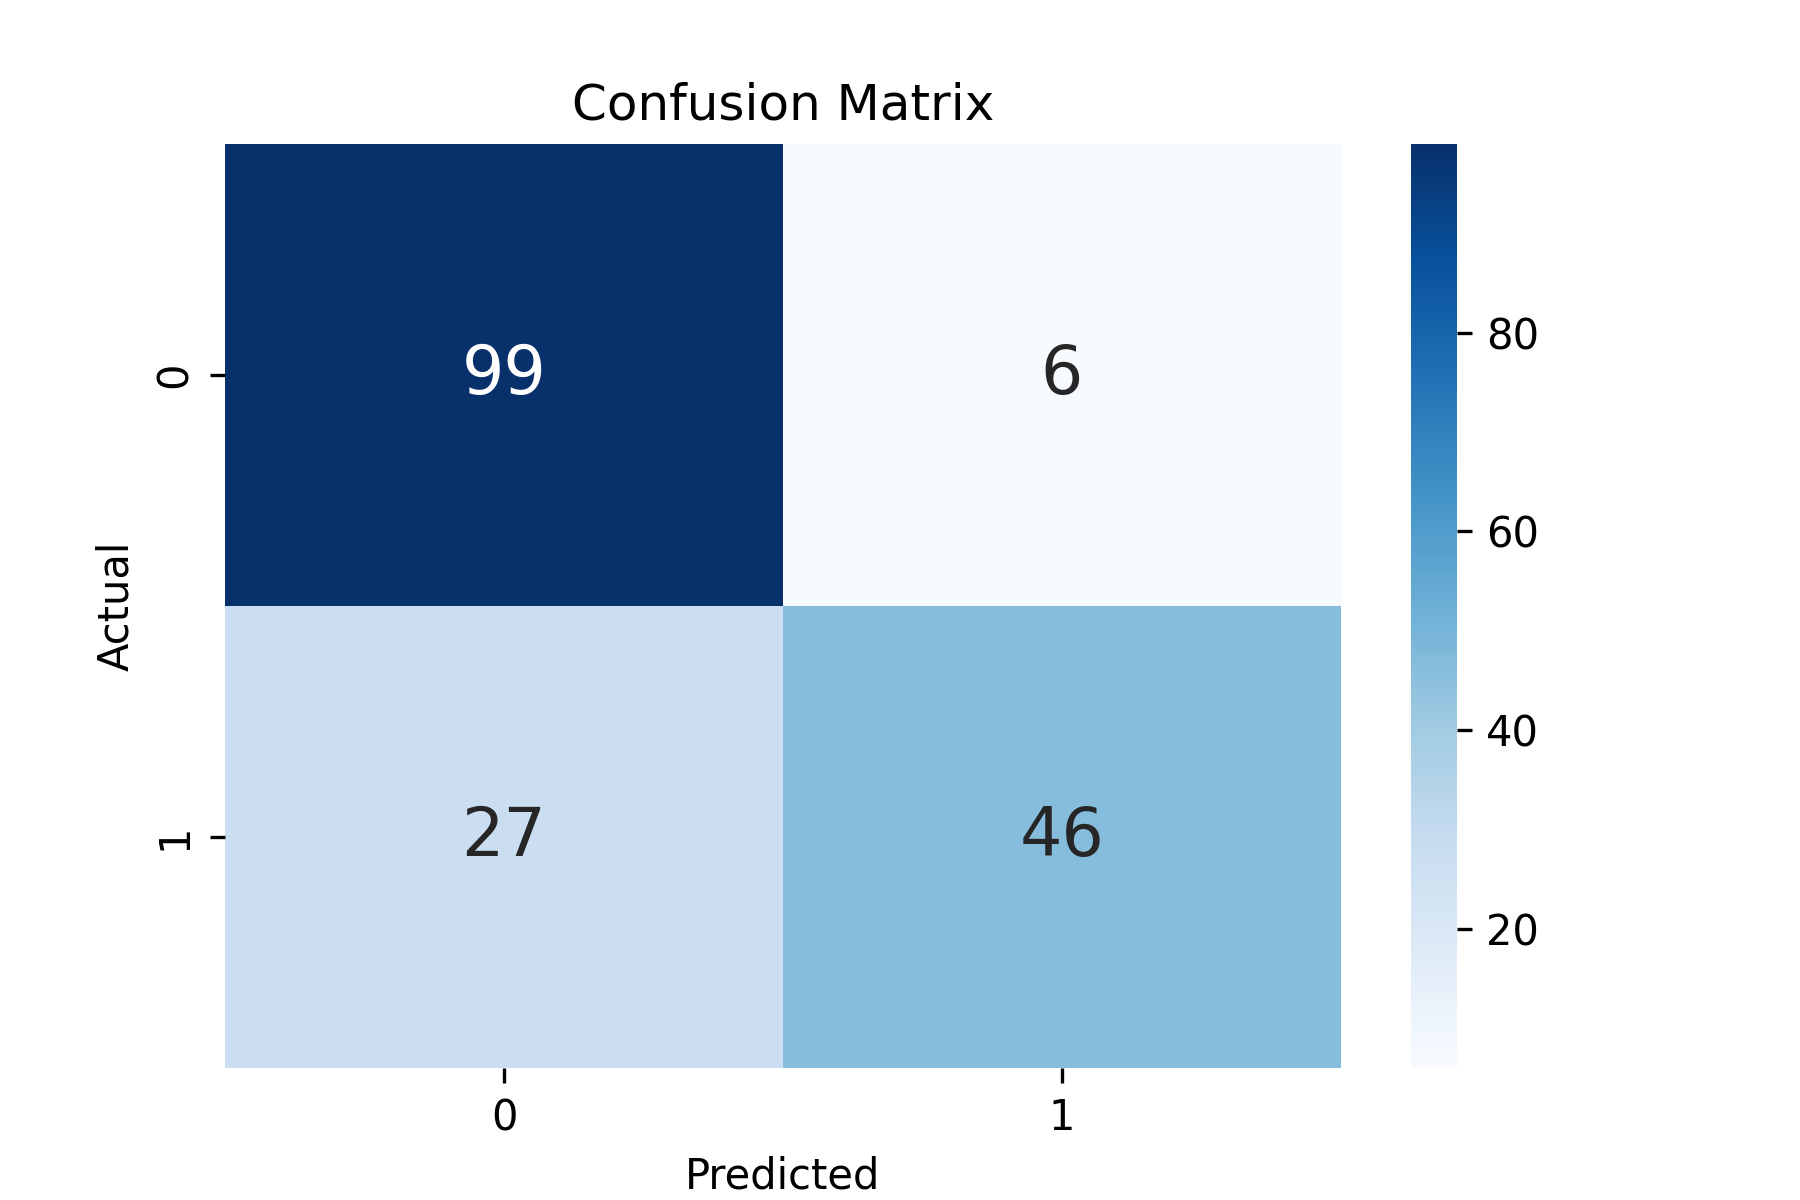
\includegraphics[width=0.7\textwidth]{../hw1/img/Part_II/confusion_matrix.png}
    \caption{Confusion matrix of the logistic regression model}
    \label{fig:confusion_matrix}
\end{figure}

The accuracy on the validation set is 0.8146. Figure \ref{fig:confusion_matrix} illustrated the confusion matrix of the logistic regression model on the validation set. The precision is 0.8846, the recall is 0.6301 and the F1 score is 0.7360. The coefficients of the model are shown in Table \ref{tab:coefficients}.

% Table for the model's parameters
\begin{table}[!htbp]
    \centering
    \begin{tabular}{@{}ll@{}}
    \toprule
    \textbf{Feature} & \textbf{Coefficient} \\ \midrule
    Pclass           & -9.937140               \\
    Age              & 31.988659               \\
    AgeXPclass       & -0.863969               \\
    IsFemale         & 63.396897                \\
    IsChild          & 9.037811                \\
    IsAlone          & 3.696076               \\
    FareGroup        & -0.611717                \\
    Embarked\_C      & 20.067069                \\
    Embarked\_Q      & 19.275919               \\
    Embarked\_S      & 11.661376               \\ \bottomrule
    \end{tabular}
    \caption{Coefficients of the logistic regression model}
    \label{tab:coefficients}
\end{table}

After training the model, the test set is loaded and preprocessed in the same way as the training set. Then, the model is used to predict the survival of passengers in the test set. The predictions are saved in a CSV file and submitted to Kaggle. The accuracy on the test set is 0.78708, which is ranked 1,331 out of 14,559+ teams on the leaderboard as in Figure \ref{fig:kaggle_leaderboard}.

% Kaggle leaderboard
\begin{figure}[!htbp]
    \centering
    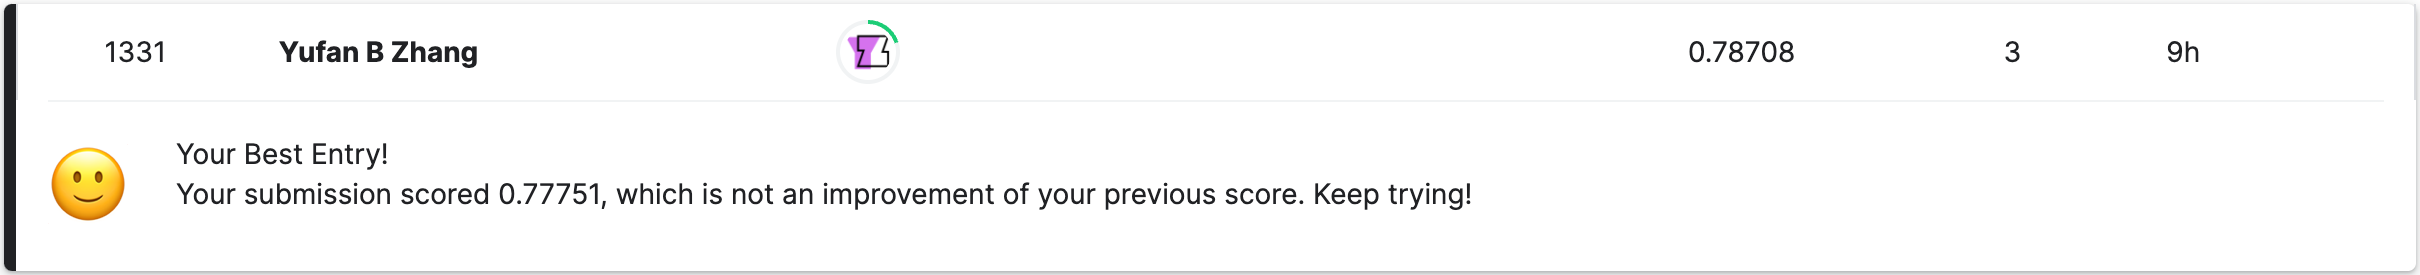
\includegraphics[width=\textwidth]{../hw1/result/Part_II/leaderboard.png}
    \caption{My Submission on Kaggle leaderboard}
    \label{fig:kaggle_leaderboard}
\end{figure}

\section{Written Exercises}

\subsection{Conceptual questions}

\subsubsection*{a. Advantages and disadvantages of gradient descent}

\textbf{Advantage:} Gradient descent is more general and can be used to optimize any objective function, whereas OLS is specific to the least squares objective function. In other words, if one wants to optimize a different objective function with no closed-form solution, gradient descent would be applicable.
    
\textbf{Disadvantage:} Gradient descent can be slower to converge than analytical formula approaches. Since the analytical formula such as OLS has a closed-form solution, it can be computed directly. However, gradient descent requires multiple iterations to converge to the optimal solution.

\subsubsection*{b. Regression by classification with discretization}

It could be a possible approach to solve the regression problem by discretizing the continuous target variable into a finite number of bins and then solving a classification problem. However, this approach has several disadvantages, which often make it insufficient in practice. 

\begin{itemize}
    \item The accuracy of the classification problem is limited by the number of bins (i.e., the number of classes). If the interval within each bin is too large, the model will not be able to predict the target variable accurately.
    \item The discretization process may introduce computational complexity to the classification problem, especially when the number of bins is large.
\end{itemize}


\subsubsection*{c. One-vs-all classification vs. multi-class classification}

\textbf{Advantage:} One-vs-all can be more useful when I have a reliable binary classifier. By applying one-vs-all, I can adapt the existing well-tuned binary classifier binary classifier to a multi-class problem.

\textbf{Disadvantage:} It can be computationally intensive if the number of classes is large. That is, I need to train $k$ binary classifiers for $k$ classes.


\subsubsection*{d. Polynomial regression}

\textbf{i. Dimension of the polynomial features}

The dimension of the polynomial features that are needed to implement this model class is \( O(p^d) \).

This is because for polynomial regression of degree \( p \) in \( d \) variables, the number of terms is given by the following formula:

\[
\binom{d+p}{p}
\]

That is, for each variable, I need to include all polynomial terms up to degree \( p \).

\textbf{ii. Computational complexity of polynomial least squares}

The computational complexity of polynomial least squares is \( O(p^{3d}) \).

To solve the normal equation, I can find the least squares solution by computing the inverse of \( X^TX \) and multiplying it with \( X^T \). The complexity of inverting a matrix is \( O(k^3) \) for a matrix of size \( k \times k \). Since \( k \) is \( O(p^d) \), the complexity becomes:

\[
O((p^d)^3) = O(p^{3d})
\]

Also, multiplying \( X^TX \) itself is \( O(n \cdot (p^d)^2) \). Therefore, the overall complexity is \( O(p^{3d}) \).

\textbf{iii. Real-world settings}

As the complexity of polynomial regression is \( O(p^{3d}) \), it might be \textbf{computationally expensive} to use it in real-world settings as the degree \( p \) or the number of attributes \( d \) increases. Also, mapping the data to a higher-dimensional space can lead to \textbf{overfitting}, which would result in poor generalization performance on unseen data. Moreover, the model might be too complex to \textbf{interpret}, which makes it less useful in practice.

Therefore, for datasets with many attributes or when a high polynomial degree is desired, it might be more practical to consider other regression methods or dimensionality reduction techniques, or to use regularization to control overfitting.


\subsection{Analytical solution for Ordinary Least Squares}

\textbf{Given:}
\begin{align*}
f_{\theta}(x^{(i)}) &= \theta_0 + \theta_1 x^{(i)} \\
J(\theta_0, \theta_1) &= \sum_{i=1}^{n} (y^{(i)} - f_{\theta}(x^{(i)}))^2
\end{align*}

\subsubsection*{a. Partial derivatives}

For \( \theta_0 \):
\begin{align*}
\frac{\partial J}{\partial \theta_0} &= \frac{\partial}{\partial \theta_0} \sum_{i=1}^{n} (y^{(i)} - \theta_0 - \theta_1 x^{(i)})^2 \\
&= -2\sum_{i=1}^{n} (y^{(i)} - \theta_0 - \theta_1 x^{(i)})
\end{align*}

For \( \theta_1 \):
\begin{align*}
\frac{\partial J}{\partial \theta_1} &= \frac{\partial}{\partial \theta_1} \sum_{i=1}^{n} (y^{(i)} - \theta_0 - \theta_1 x^{(i)})^2 \\
&= -2\sum_{i=1}^{n} (y^{(i)} - \theta_0 - \theta_1 x^{(i)}) x^{(i)}
\end{align*}

\subsubsection*{b. Using the normal equations}

For \( \theta_0 \), setting the gradient to zero:
\begin{align*}
\sum_{i=1}^{n} (y^{(i)} - \theta_0 - \theta_1 x^{(i)}) &= 0 \\
\Rightarrow n\bar{y} &= n\theta_0 + \theta_1 \sum_{i=1}^{n} x^{(i)}
\end{align*}

For \( \theta_1 \), setting the gradient to zero:
\begin{align*}
\sum_{i=1}^{n} (y^{(i)} - \theta_0 - \theta_1 x^{(i)}) x^{(i)} &= 0 \\
\Rightarrow \theta_1 &= \frac{\sum_{i=1}^{n} (x^{(i)} - \bar{x})(y^{(i)} - \bar{y})}{\sum_{i=1}^{n} (x^{(i)} - \bar{x})^2}
\end{align*}

Using the derived value of \( \theta_1 \), I can substitute it into the equation for \( \theta_0 \):

\begin{align*}
n\bar{y} &= n\theta_0 + \frac{\sum_{i=1}^{n} (x^{(i)} - \bar{x})(y^{(i)} - \bar{y})}{\sum_{i=1}^{n} (x^{(i)} - \bar{x})^2} \sum_{i=1}^{n} x^{(i)} \\
\Rightarrow \theta_0 &= \bar{y} - \frac{\sum_{i=1}^{n} (x^{(i)} - \bar{x})(y^{(i)} - \bar{y})}{\sum_{i=1}^{n} (x^{(i)} - \bar{x})^2} \bar{x}
\end{align*}

Therefore, I can deduce:
\[ \theta_0 = \bar{y} - \theta_1 \bar{x} \]

\subsubsection*{c. Sum of residuals for optimal parameters}

Given:
\[ e^{(i)} = y^{(i)} - (\theta_0^* + \theta_1^* x^{(i)}) \]
Summing over all residuals:
\[ \sum_{i=1}^{n} e^{(i)} = \sum_{i=1}^{n} (y^{(i)} - \theta_0^* - \theta_1^* x^{(i)}) \]

From the normal equations, the sum of residuals will be zero, which indicates that the best-fit line passes through the mean of the data points (i.e. \((\bar{x}, \bar{y})\)). Moreover, the deviations above the regression line are balanced out by the deviations below the line on average.


\subsection{Maximum Likelihood Estimation}

\subsubsection*{a. Probabilistic model and learning paradigm}

\textbf{i. Probabilistic model:}

Let \(p_i\) denote the denote the probability that the dice falls on side \(i\). I can define out probabilistic model as the probabilities \(p_1, p_2, p_3\), and \(p_4\). Also, I have the following constraints:

\begin{align*}
p_1 + p_2 + p_3 + p_4 &= 1 \\
p_i &\geq 0 \quad \forall i \in \{1, 2, 3, 4\}
\end{align*}

\textbf{ii. Learning paradigm:}

The learning paradigm for this problem is \textbf{unsupervised learning} since I do not have any labels for the data (i.e., the true probabilities of each side of the dice). Therefore, I need to learn the parameters of the model from the data without any supervision.

\subsubsection*{b. Log-likelihood of the dataset}

Each dice throw is independent and identically distributed (i.i.d.). Then, the likelihood of observing a sequence of \(n\) dice throws is given by the product of the probabilities of each individual dice throw:

\[
\mathcal{L}(\theta) = \prod_{i=1}^{n} p_{x_i}
\]

Taking the log on both sides, the log-likelihood is:

\[
\log \mathcal{L}(\theta) = \sum_{i=1}^{n} \log p_{x_i}
\]

\textbf{Intuitive argument:} An intuitive reason to optimize the log-likelihood instead of the likelihood is that taking the log transforms the product into a sum, which is numerically more stable and also makes the differentiation easier.


\subsubsection*{c. Maximum likelihood estimation}

In the case of this dice toss problem, MLEs are the values of \(p_1, p_2, p_3\), and \(p_4\) that maximize the log-likelihood, which yields the frequencies of each side of the dice. That is:

\[
\hat{p}_i = \frac{\text{number of times side } i \text{ appears}}{n}
\]

Given the data in the table, we can compute the MLEs as follows:

\begin{align*}
\hat{p}_1 &= 0 \\
\hat{p}_2 &= \frac{2}{8} = 0.25 \\
\hat{p}_3 &= \frac{2}{8} = 0.25 \\
\hat{p}_4 &= \frac{4}{8} = 0.5
\end{align*}

This means, based on our observations, we estimate that the probabilities of the dice landing on sides 1, 2, 3, and 4 are 0, 0.25, 0.25, and 0.5 respectively.

\subsubsection*{d. Potential inaccuracies}

Scenarios where this approach might yield inaccurate estimates:

\begin{itemize}
    \item The number of dice throws is too small. In this case, the estimates might be inaccurate because the sample may not be representative of the true probabilities.
    \item The dice is not thrown randomly. In this case, the estimates might be inaccurate because the throws are not i.i.d.
\end{itemize}

\textbf{Examples:} If I throw the fair dice only 2 times and get the outcome sequence {1, 1}, the MLE would be \(\hat{p}_1 = 1\) and 0 for all other sides. However, this is clearly not a good estimate of the true probabilities. That is, the sample is too small to be representative of the true probabilities.

\printbibliography

\end{document}
